\documentclass[12pt,a4paper]{article}

% --- CHÚ Ý QUAN TRỌNG ĐỂ KHÔNG BỊ LỖI ---
% 1. Đã vô hiệu hóa gói ex_test để tránh lỗi thiếu file (Bỏ % nếu bạn có file ex_test.sty)
% \usepackage[solcolor]{ex_test} 

% 2. Lệnh này giúp fix triệt để lỗi copy/paste dính khoảng trắng tàng hình (U+00A0)
\DeclareUnicodeCharacter{00A0}{ }

% --- Các gói cơ bản cho khoa học, toán học và định dạng ---
\usepackage[utf8]{inputenc}
\usepackage[T5]{fontenc} 
\usepackage{mathptmx} 
\usepackage{amsmath,amssymb,amsfonts,yhmath}
\usepackage{enumitem}

% Căn lề chuẩn Đồ án
\usepackage[top=2cm, bottom=2cm, left=3cm, right=2cm]{geometry} 

% Giãn dòng 1.5
\usepackage{setspace}
\onehalfspacing 
\usepackage[table]{xcolor}
\definecolor{uehred}{RGB}{210, 50, 40}
\usepackage[hidelinks,unicode]{hyperref}
\usepackage{titlesec}
\usepackage{sectsty}

% Hỗ trợ bảng 
\usepackage{float}
\usepackage{booktabs}
\usepackage{longtable}
\usepackage{array}
\usepackage{graphicx}
\usepackage{listings}
\usepackage{minted}
\setminted{
    fontsize=\small,
    breaklines=true,
    frame=single,
    autogobble=true
}
\usepackage[most]{tcolorbox}
\tcbuselibrary{listings}

% --- Các gói bổ sung cho trang bìa UEH ---
\usepackage{tikz}        
\usetikzlibrary{calc,positioning,arrows.meta,shapes.multipart,fit}
\usepackage{anyfontsize}
\usepackage{helvet}      

% Định nghĩa màu sắc thương hiệu UEH
\definecolor{uehteal}{HTML}{2D5D66}   
\definecolor{uehorange}{HTML}{D96B42} 
\definecolor{uehblue}{HTML}{1A408B}   

% Thụt đầu dòng
\usepackage{indentfirst}
\setlength{\parindent}{1.27cm} 

% Việt hóa các tiêu đề
\renewcommand{\contentsname}{Mục lục}
\renewcommand{\figurename}{Hình}
\renewcommand{\tablename}{Bảng}
\renewcommand{\refname}{Tài liệu tham khảo}

% Định dạng lại font chữ
\sectionfont{\Large\bfseries}
\subsectionfont{\large\bfseries}

\usepackage{fontawesome5}

% Bỏ header và footer
\pagestyle{empty}

% --- Các lệnh custom toán học ---
\renewcommand{\ge}{\geqslant}
\renewcommand{\geq}{\geqslant}
\renewcommand{\le}{\leqslant}
\renewcommand{\leq}{\leqslant}
\newcommand{\tron}[1]{\left( #1 \right)}
\newcommand{\vuong}[1]{\left[ #1 \right]}
\newcommand{\nhon}[1]{\left\{ #1 \right\}}
\newcommand{\sieuto}[1]{\Big( #1 \Big)}

%% vsc 

% --- BỘ MÀU VS CODE DARK+ CHUẨN ---
\definecolor{vs_bg}{HTML}{1E1E1E}       % Nền tối
\definecolor{vs_fg}{HTML}{D4D4D4}       % Chữ thường (Trắng xám)
\definecolor{vs_keyword}{HTML}{569CD6}  % Từ khóa (Xanh dương: public, void, string...)
\definecolor{vs_control}{HTML}{C586C0}  % Điều kiện (Tím hồng: if, return...)
\definecolor{vs_type}{HTML}{4EC9B0}     % Class/Struct (Xanh ngọc: Console, Student...)
\definecolor{vs_function}{HTML}{DCDCAA} % Hàm (Vàng nhạt: WriteLine, Main...)
\definecolor{vs_string}{HTML}{CE9178}   % Chuỗi (Cam đất)
\definecolor{vs_comment}{HTML}{6A9955}  % Comment (Xanh lá)
\definecolor{vs_number}{HTML}{B5CEA8}   % Số (Xanh lá mạ)
\definecolor{vs_variable}{HTML}{9CDCFE} % Biến/Tham số (Xanh da trời nhạt: args, st...)

\newcommand{\vno}{\mbox{o}}
\newcommand{\vnohorn}{\mbox{\protect\horn{o}}}
\newcommand{\vnohornac}{\mbox{\protect\'{\protect\horn{o}}}}
\newcommand{\vnohorngr}{\mbox{\protect\`{\protect\horn{o}}}}
\newcommand{\vnohornhk}{\mbox{\protect\h{\protect\horn{o}}}}
\newcommand{\vnohorntd}{\mbox{\protect\~{\protect\horn{o}}}}
\newcommand{\vnohorndt}{\mbox{\protect\d{\protect\horn{o}}}}
% (Các ký tự Râu Ư)
\newcommand{\vnuhorn}{\mbox{\protect\horn{u}}}
\newcommand{\vnuhornac}{\mbox{\protect\'{\protect\horn{u}}}}
\newcommand{\vnuhorngr}{\mbox{\protect\`{\protect\horn{u}}}}
\newcommand{\vnuhornhk}{\mbox{\protect\h{\protect\horn{u}}}}
\newcommand{\vnuhorntd}{\mbox{\protect\~{\protect\horn{u}}}}
\newcommand{\vnuhorndt}{\mbox{\protect\d{\protect\horn{u}}}}
% (Các ký tự Râu Hoa Ơ, Ư)
\newcommand{\vnOHORN}{\mbox{\protect\horn{O}}} \newcommand{\vnOHORNAC}{\mbox{\protect\'{\protect\horn{O}}}} \newcommand{\vnOHORNGR}{\mbox{\protect\`{\protect\horn{O}}}} \newcommand{\vnOHORNHK}{\mbox{\protect\h{\protect\horn{O}}}} \newcommand{\vnOHORNTD}{\mbox{\protect\~{\protect\horn{O}}}} \newcommand{\vnOHORNDT}{\mbox{\protect\d{\protect\horn{O}}}}
\newcommand{\vnUHORN}{\mbox{\protect\horn{U}}} \newcommand{\vnUHORNAC}{\mbox{\protect\'{\protect\horn{U}}}} \newcommand{\vnUHORNGR}{\mbox{\protect\`{\protect\horn{U}}}} \newcommand{\vnUHORNHK}{\mbox{\protect\h{\protect\horn{U}}}} \newcommand{\vnUHORNTD}{\mbox{\protect\~{\protect\horn{U}}}} \newcommand{\vnUHORNDT}{\mbox{\protect\d{\protect\horn{U}}}}
% (Các ký tự Mũ Â, Ê, Ô)   
\newcommand{\vnacirc}{\mbox{\protect\^a}} \newcommand{\vnacircac}{\mbox{\protect\'{\protect\^a}}} \newcommand{\vnacircgr}{\mbox{\protect\`{\protect\^a}}} \newcommand{\vnacirchk}{\mbox{\protect\h{\protect\^a}}} \newcommand{\vnacirctd}{\mbox{\protect\~{\protect\^a}}} \newcommand{\vnacircdt}{\mbox{\protect\d{\protect\^a}}}
\newcommand{\vnecirc}{\mbox{\protect\^e}} \newcommand{\vnecircac}{\mbox{\protect\'{\protect\^e}}} \newcommand{\vnecircgr}{\mbox{\protect\`{\protect\^e}}} \newcommand{\vnecirchk}{\mbox{\protect\h{\protect\^e}}} \newcommand{\vnecirctd}{\mbox{\protect\~{\protect\^e}}} \newcommand{\vnecircdt}{\mbox{\protect\d{\protect\^e}}}
\newcommand{\vnocirc}{\mbox{\protect\^o}} \newcommand{\vnocircac}{\mbox{\protect\'{\protect\^o}}} \newcommand{\vnocircgr}{\mbox{\protect\`{\protect\^o}}} \newcommand{\vnocirchk}{\mbox{\protect\h{\protect\^o}}} \newcommand{\vnocirctd}{\mbox{\protect\~{\protect\^o}}} \newcommand{\vnocircdt}{\mbox{\protect\d{\protect\^o}}}
\newcommand{\vnACIRC}{\mbox{\protect\^A}} \newcommand{\vnACIRCAC}{\mbox{\protect\'{\protect\^A}}} \newcommand{\vnACIRCGR}{\mbox{\protect\`{\protect\^A}}} \newcommand{\vnACIRCHK}{\mbox{\protect\h{\protect\^A}}} \newcommand{\vnACIRCTD}{\mbox{\protect\~{\protect\^A}}} \newcommand{\vnACIRCDT}{\mbox{\protect\d{\protect\^A}}}
\newcommand{\vnECIRC}{\mbox{\protect\^E}} \newcommand{\vnECIRCAC}{\mbox{\protect\'{\protect\^E}}} \newcommand{\vnECIRCGR}{\mbox{\protect\`{\protect\^E}}} \newcommand{\vnECIRCHK}{\mbox{\protect\h{\protect\^E}}} \newcommand{\vnECIRCTD}{\mbox{\protect\~{\protect\^E}}} \newcommand{\vnECIRCDT}{\mbox{\protect\d{\protect\^E}}}
\newcommand{\vnOCIRC}{\mbox{\protect\^O}} \newcommand{\vnOCIRCAC}{\mbox{\protect\'{\protect\^O}}} \newcommand{\vnOCIRCGR}{\mbox{\protect\`{\protect\^O}}} \newcommand{\vnOCIRCHK}{\mbox{\protect\h{\protect\^O}}} \newcommand{\vnOCIRCTD}{\mbox{\protect\~{\protect\^O}}} \newcommand{\vnOCIRCDT}{\mbox{\protect\d{\protect\^O}}}
% (Các ký tự Trăng Ă)
\newcommand{\vnabreve}{\mbox{\protect\u{a}}} \newcommand{\vnabreveac}{\mbox{\protect\'{\protect\u{a}}}} \newcommand{\vnabrevegr}{\mbox{\protect\`{\protect\u{a}}}} \newcommand{\vnabrevehk}{\mbox{\protect\h{\protect\u{a}}}} \newcommand{\vnabrevetd}{\mbox{\protect\~{\protect\u{a}}}} \newcommand{\vnabrevedt}{\mbox{\protect\d{\protect\u{a}}}}
\newcommand{\vnABREVE}{\mbox{\protect\u{A}}} \newcommand{\vnABREVEAC}{\mbox{\protect\'{\protect\u{A}}}} \newcommand{\vnABREVEGR}{\mbox{\protect\`{\protect\u{A}}}} \newcommand{\vnABREVEHK}{\mbox{\protect\h{\protect\u{A}}}} \newcommand{\vnABREVETD}{\mbox{\protect\~{\protect\u{A}}}} \newcommand{\vnABREVEDT}{\mbox{\protect\d{\protect\u{A}}}}
% (Các ký tự Đơn)
\newcommand{\vnaac}{\mbox{\protect\'a}} \newcommand{\vnagr}{\mbox{\protect\`a}} \newcommand{\vnahk}{\mbox{\protect\h{a}}} \newcommand{\vnatd}{\mbox{\protect\~a}} \newcommand{\vnadt}{\mbox{\protect\d{a}}}
\newcommand{\vnAAC}{\mbox{\protect\'A}} \newcommand{\vnAGR}{\mbox{\protect\`A}} \newcommand{\vnAHK}{\mbox{\protect\h{A}}} \newcommand{\vnATD}{\mbox{\protect\~A}} \newcommand{\vnADT}{\mbox{\protect\d{A}}}
\newcommand{\vneac}{\mbox{\protect\'e}} \newcommand{\vnegr}{\mbox{\protect\`e}} \newcommand{\vnehk}{\mbox{\protect\h{e}}} \newcommand{\vnetd}{\mbox{\protect\~e}} \newcommand{\vnedt}{\mbox{\protect\d{e}}}
\newcommand{\vnEAC}{\mbox{\protect\'E}} \newcommand{\vnEGR}{\mbox{\protect\`E}} \newcommand{\vnEHK}{\mbox{\protect\h{E}}} \newcommand{\vnETD}{\mbox{\protect\~E}} \newcommand{\vnEDT}{\mbox{\protect\d{E}}}
\newcommand{\vniac}{\mbox{\protect\'i}} \newcommand{\vnigr}{\mbox{\protect\`i}} \newcommand{\vnihk}{\mbox{\protect\h{i}}} \newcommand{\vnitd}{\mbox{\protect\~i}} \newcommand{\vnidt}{\mbox{\protect\d{i}}}
\newcommand{\vnIAC}{\mbox{\protect\'I}} \newcommand{\vnIGR}{\mbox{\protect\`I}} \newcommand{\vnIHK}{\mbox{\protect\h{I}}} \newcommand{\vnITD}{\mbox{\protect\~I}} \newcommand{\vnIDT}{\mbox{\protect\d{I}}}
\newcommand{\vnoac}{\mbox{\protect\'o}} \newcommand{\vnogr}{\mbox{\protect\`o}} \newcommand{\vnohk}{\mbox{\protect\h{o}}} \newcommand{\vnotd}{\mbox{\protect\~o}} \newcommand{\vnodt}{\mbox{\protect\d{o}}}
\newcommand{\vnOAC}{\mbox{\protect\'O}} \newcommand{\vnOGR}{\mbox{\protect\`O}} \newcommand{\vnOHK}{\mbox{\protect\h{O}}} \newcommand{\vnOTD}{\mbox{\protect\~O}} \newcommand{\vnODT}{\mbox{\protect\d{O}}}
\newcommand{\vnuac}{\mbox{\protect\'u}} \newcommand{\vnugr}{\mbox{\protect\`u}} \newcommand{\vnuhk}{\mbox{\protect\h{u}}} \newcommand{\vnutd}{\mbox{\protect\~u}} \newcommand{\vnudt}{\mbox{\protect\d{u}}}
\newcommand{\vnUAC}{\mbox{\protect\'U}} \newcommand{\vnUGR}{\mbox{\protect\`U}} \newcommand{\vnUHK}{\mbox{\protect\h{U}}} \newcommand{\vnUTD}{\mbox{\protect\~U}} \newcommand{\vnUDT}{\mbox{\protect\d{U}}}
\newcommand{\vnyac}{\mbox{\protect\'y}} \newcommand{\vnygr}{\mbox{\protect\`y}} \newcommand{\vnyhk}{\mbox{\protect\h{y}}} \newcommand{\vnytd}{\mbox{\protect\~y}} \newcommand{\vnydt}{\mbox{\protect\d{y}}}
\newcommand{\vnYAC}{\mbox{\protect\'Y}} \newcommand{\vnYGR}{\mbox{\protect\`Y}} \newcommand{\vnYHK}{\mbox{\protect\h{Y}}} \newcommand{\vnYTD}{\mbox{\protect\~Y}} \newcommand{\vnYDT}{\mbox{\protect\d{Y}}}
\newcommand{\vndd}{\mbox{\protect\dj}}  \newcommand{\vnDD}{\mbox{\protect\DJ}}

% --- 4. CẤU HÌNH STYLE CODE ---
\lstdefinestyle{vs_style}{
	language=C++,
	basicstyle=\ttfamily\small\color{vs_fg},
	columns=fullflexible,
	% 1. Từ khóa chính (Xanh dương)
	keywords=[1]{int, float, void, bool, true, false, using, namespace, class, public, return, private},
	keywordstyle=[1]\color{vs_keyword}\bfseries,
	% 2. Từ khóa điều kiện/luồng (Hồng tím)
	keywords=[2]{if, else, for, while, switch, case, break, include, define},
	keywordstyle=[2]\color{vs_control}\bfseries,
	% 3. Thư viện (Cam đất)
	keywords=[3]{iostream, vector, string, cout, cin},
	keywordstyle=[3]\color{vs_string}\bfseries,
	% Comment & String
	commentstyle=\color{vs_comment}\itshape,
	identifierstyle=\color{white},
	stringstyle=\color{vs_string},
	% Số dòng
	numbers=left,
	numbersep=5pt,
	xleftmargin=1.5em,
	breaklines=true,
	breakindent=2em,
	postbreak=\mbox{\textcolor{gray}{$\hookrightarrow$}\space},
	showstringspaces=false,
	tabsize=2,
	% --- LITERATE: QUAN TRỌNG NHẤT ĐỂ TÔ MÀU DẤU ---
	literate={
		% Tiếng Việt
		{ơ}{{\vnohorn}}1 {ớ}{{\vnohornac}}1 {ờ}{{\vnohorngr}}1 {ở}{{\vnohornhk}}1 {ỡ}{{\vnohorntd}}1 {ợ}{{\vnohorndt}}1
		{Ơ}{{\vnOHORN}}1 {Ớ}{{\vnOHORNAC}}1 {Ờ}{{\vnOHORNGR}}1 {Ở}{{\vnOHORNHK}}1 {Ỡ}{{\vnOHORNTD}}1 {Ợ}{{\vnOHORNDT}}1
		{ư}{{\vnuhorn}}1 {ứ}{{\vnuhornac}}1 {ừ}{{\vnuhorngr}}1 {ử}{{\vnuhornhk}}1 {ữ}{{\vnuhorntd}}1 {ự}{{\vnuhorndt}}1
		{Ư}{{\vnUHORN}}1 {Ứ}{{\vnUHORNAC}}1 {Ừ}{{\vnUHORNGR}}1 {Ử}{{\vnUHORNHK}}1 {Ữ}{{\vnUHORNTD}}1 {Ự}{{\vnUHORNDT}}1
		{â}{{\vnacirc}}1 {ấ}{{\vnacircac}}1 {ầ}{{\vnacircgr}}1 {ẩ}{{\vnacirchk}}1 {ẫ}{{\vnacirctd}}1 {ậ}{{\vnacircdt}}1
		{Â}{{\vnACIRC}}1 {Ấ}{{\vnACIRCAC}}1 {Ầ}{{\vnACIRCGR}}1 {Ẩ}{{\vnACIRCHK}}1 {Ẫ}{{\vnACIRCTD}}1 {Ậ}{{\vnACIRCDT}}1
		{ê}{{\vnecirc}}1 {ế}{{\vnecircac}}1 {ề}{{\vnecircgr}}1 {ể}{{\vnecirchk}}1 {ễ}{{\vnecirctd}}1 {ệ}{{\vnecircdt}}1
		{Ê}{{\vnECIRC}}1 {Ế}{{\vnECIRCAC}}1 {Ề}{{\vnECIRCGR}}1 {Ể}{{\vnECIRCHK}}1 {Ễ}{{\vnECIRCTD}}1 {Ệ}{{\vnECIRCDT}}1
		{ô}{{\vnocirc}}1 {ố}{{\vnocircac}}1 {ồ}{{\vnocircgr}}1 {ổ}{{\vnocirchk}}1 {ỗ}{{\vnocirctd}}1 {ộ}{{\vnocircdt}}1
		{Ô}{{\vnOCIRC}}1 {Ố}{{\vnOCIRCAC}}1 {Ồ}{{\vnOCIRCGR}}1 {Ổ}{{\vnOCIRCHK}}1 {Ỗ}{{\vnOCIRCTD}}1 {Ộ}{{\vnOCIRCDT}}1
		{ă}{{\vnabreve}}1 {ắ}{{\vnabreveac}}1 {ằ}{{\vnabrevegr}}1 {ẳ}{{\vnabrevehk}}1 {ẵ}{{\vnabrevetd}}1 {ặ}{{\vnabrevedt}}1
		{Ă}{{\vnABREVE}}1 {Ắ}{{\vnABREVEAC}}1 {Ằ}{{\vnABREVEGR}}1 {Ẳ}{{\vnABREVEHK}}1 {Ẵ}{{\vnABREVETD}}1 {Ặ}{{\vnABREVEDT}}1
		{đ}{{\vndd}}1 {Đ}{{\vnDD}}1
		{á}{{\vnaac}}1 {à}{{\vnagr}}1 {ả}{{\vnahk}}1 {ã}{{\vnatd}}1 {ạ}{{\vnadt}}1
		{Á}{{\vnAAC}}1 {À}{{\vnAGR}}1 {Ả}{{\vnAHK}}1 {Ã}{{\vnATD}}1 {Ạ}{{\vnADT}}1
		{é}{{\vneac}}1 {è}{{\vnegr}}1 {ẻ}{{\vnehk}}1 {ẽ}{{\vnetd}}1 {ẹ}{{\vnedt}}1
		{É}{{\vnEAC}}1 {È}{{\vnEGR}}1 {Ẻ}{{\vnEHK}}1 {Ẽ}{{\vnETD}}1 {Ẹ}{{\vnEDT}}1
		{í}{{\vniac}}1 {ì}{{\vnigr}}1 {ỉ}{{\vnihk}}1 {ĩ}{{\vnitd}}1 {ị}{{\vnidt}}1
		{Í}{{\vnIAC}}1 {Ì}{{\vnIGR}}1 {Ỉ}{{\vnIHK}}1 {Ĩ}{{\vnITD}}1 {Ị}{{\vnIDT}}1
		{ó}{{\vnoac}}1 {ò}{{\vnogr}}1 {ỏ}{{\vnohk}}1 {õ}{{\vnotd}}1 {ọ}{{\vnodt}}1
		{Ó}{{\vnOAC}}1 {Ò}{{\vnOGR}}1 {Ỏ}{{\vnOHK}}1 {Õ}{{\vnOTD}}1 {Ọ}{{\vnODT}}1
		{ú}{{\vnuac}}1 {ù}{{\vnugr}}1 {ủ}{{\vnuhk}}1 {ũ}{{\vnutd}}1 {ụ}{{\vnudt}}1
		{Ú}{{\vnUAC}}1 {Ù}{{\vnUGR}}1 {Ủ}{{\vnUHK}}1 {Ũ}{{\vnUTD}}1 {Ụ}{{\vnUDT}}1
		{ý}{{\vnyac}}1 {ỳ}{{\vnygr}}1 {ỷ}{{\vnyhk}}1 {ỹ}{{\vnytd}}1 {ỵ}{{\vnydt}}1
		{Ý}{{\vnYAC}}1 {Ỳ}{{\vnYGR}}1 {Ỷ}{{\vnYHK}}1 {Ỹ}{{\vnYTD}}1 {Ỵ}{{\vnYDT}}1
		{~}{{$\sim$}}1
		% --- SỬA LỖI PARAMETER (Dấu \#) ---
		{\#}{{\textcolor{vs_control}{\#}}}1  
		{\\}{{\textcolor{vs_control}{\textbackslash}}}1 
	} 
}

% --- 5. TẠO BOX ---
\newtcblisting[auto counter]{vscode}[2][]{
	enhanced,
	breakable,
	colback=vs_bg,
	colframe=gray!40!black, 
	coltitle=vs_fg,
	fonttitle=\bfseries\sffamily\small,
	title={
		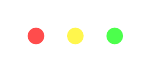
\begin{tikzpicture}[baseline={(0,-0.1)}]
			\fill[red!70] (0,-0.2) circle (3pt);
			\fill[yellow!70] (0.5,-0.2) circle (3pt);
			\fill[green!70] (1.0,-0.2) circle (3pt);
		\end{tikzpicture}
	},
	arc=4mm,
	boxrule=0.5pt,
	left=2mm, right=2mm, top=1mm, bottom=1mm,
	listing only,
	coltext=vs_fg,      
	colupper=vs_fg,     
	listing style=vs_style,
	#1
}

% --- 6. STYLE C# (CSHARP) ---
\lstdefinestyle{cs_style}{
	language=[Sharp]C, 
	basicstyle=\ttfamily\small\color{vs_fg},
	columns=fullflexible,
    keywords=[1]{using, namespace, public, private, protected, internal, static, void, int, string, float, double, bool, var, new, true, false, null, out, ref, struct, class},
	keywordstyle=[1]\color{vs_keyword}\bfseries,
	keywords=[2]{if, else, for, foreach, while, switch, case, break, return, try, catch},
	keywordstyle=[2]\color{vs_control}\bfseries,
	keywords=[3]{Console, Program, Student, System, Exception, Math, List, DateTime},
	keywordstyle=[3]\color{vs_string}\bfseries,
    keywords=[4]{WriteLine, Write, ReadLine, Parse, ToString, NhapSV, XuatSV, Main},
    keywordstyle=[4]\color{vs_function},
    keywords=[5]{st, args},
    keywordstyle=[5]\color{vs_variable},
    commentstyle=\color{vs_comment}\itshape,
    stringstyle=\color{vs_string},
    numberstyle=\color{gray!50}\small, 
	numbers=left,
	numbersep=5pt,
	xleftmargin=1.5em,
	breaklines=true,
	breakindent=2em,
	postbreak=\mbox{\textcolor{gray}{$\hookrightarrow$}\space},
	showstringspaces=false,
	tabsize=4,
	literate={
		{ơ}{{\vnohorn}}1 {ớ}{{\vnohornac}}1 {ờ}{{\vnohorngr}}1 {ở}{{\vnohornhk}}1 {ỡ}{{\vnohorntd}}1 {ợ}{{\vnohorndt}}1
		{Ơ}{{\vnOHORN}}1 {Ớ}{{\vnOHORNAC}}1 {Ờ}{{\vnOHORNGR}}1 {Ở}{{\vnOHORNHK}}1 {Ỡ}{{\vnOHORNTD}}1 {Ợ}{{\vnOHORNDT}}1
		{ư}{{\vnuhorn}}1 {ứ}{{\vnuhornac}}1 {ừ}{{\vnuhorngr}}1 {ử}{{\vnuhornhk}}1 {ữ}{{\vnuhorntd}}1 {ự}{{\vnuhorndt}}1
		{Ư}{{\vnUHORN}}1 {Ứ}{{\vnUHORNAC}}1 {Ừ}{{\vnUHORNGR}}1 {Ử}{{\vnUHORNHK}}1 {Ữ}{{\vnUHORNTD}}1 {Ự}{{\vnUHORNDT}}1
		{â}{{\vnacirc}}1 {ấ}{{\vnacircac}}1 {ầ}{{\vnacircgr}}1 {ẩ}{{\vnacirchk}}1 {ẫ}{{\vnacirctd}}1 {ậ}{{\vnacircdt}}1
		{Â}{{\vnACIRC}}1 {Ấ}{{\vnACIRCAC}}1 {Ầ}{{\vnACIRCGR}}1 {Ẩ}{{\vnACIRCHK}}1 {Ẫ}{{\vnACIRCTD}}1 {Ậ}{{\vnACIRCDT}}1
		{ê}{{\vnecirc}}1 {ế}{{\vnecircac}}1 {ề}{{\vnecircgr}}1 {ể}{{\vnecirchk}}1 {ễ}{{\vnecirctd}}1 {ệ}{{\vnecircdt}}1
		{Ê}{{\vnECIRC}}1 {Ế}{{\vnECIRCAC}}1 {Ề}{{\vnECIRCGR}}1 {Ể}{{\vnECIRCHK}}1 {Ễ}{{\vnECIRCTD}}1 {Ệ}{{\vnECIRCDT}}1
		{ô}{{\vnocirc}}1 {ố}{{\vnocircac}}1 {ồ}{{\vnocircgr}}1 {ổ}{{\vnocirchk}}1 {ỗ}{{\vnocirctd}}1 {ộ}{{\vnocircdt}}1
		{Ô}{{\vnOCIRC}}1 {Ố}{{\vnOCIRCAC}}1 {Ồ}{{\vnOCIRCGR}}1 {Ổ}{{\vnOCIRCHK}}1 {Ỗ}{{\vnOCIRCTD}}1 {Ộ}{{\vnOCIRCDT}}1
		{ă}{{\vnabreve}}1 {ắ}{{\vnabreveac}}1 {ằ}{{\vnabrevegr}}1 {ẳ}{{\vnabrevehk}}1 {ẵ}{{\vnabrevetd}}1 {ặ}{{\vnabrevedt}}1
		{Ă}{{\vnABREVE}}1 {Ắ}{{\vnABREVEAC}}1 {Ằ}{{\vnABREVEGR}}1 {Ẳ}{{\vnABREVEHK}}1 {Ẵ}{{\vnABREVETD}}1 {Ặ}{{\vnABREVEDT}}1
		{đ}{{\vndd}}1 {Đ}{{\vnDD}}1
		{á}{{\vnaac}}1 {à}{{\vnagr}}1 {ả}{{\vnahk}}1 {ã}{{\vnatd}}1 {ạ}{{\vnadt}}1
		{Á}{{\vnAAC}}1 {À}{{\vnAGR}}1 {Ả}{{\vnAHK}}1 {Ã}{{\vnATD}}1 {Ạ}{{\vnADT}}1
		{é}{{\vneac}}1 {è}{{\vnegr}}1 {ẻ}{{\vnehk}}1 {ẽ}{{\vnetd}}1 {ẹ}{{\vnedt}}1
		{É}{{\vnEAC}}1 {È}{{\vnEGR}}1 {Ẻ}{{\vnEHK}}1 {Ẽ}{{\vnETD}}1 {Ẹ}{{\vnEDT}}1
		{í}{{\vniac}}1 {ì}{{\vnigr}}1 {ỉ}{{\vnihk}}1 {ĩ}{{\vnitd}}1 {ị}{{\vnidt}}1
		{Í}{{\vnIAC}}1 {Ì}{{\vnIGR}}1 {Ỉ}{{\vnIHK}}1 {Ĩ}{{\vnITD}}1 {Ị}{{\vnIDT}}1
		{ó}{{\vnoac}}1 {ò}{{\vnogr}}1 {ỏ}{{\vnohk}}1 {õ}{{\vnotd}}1 {ọ}{{\vnodt}}1
		{Ó}{{\vnOAC}}1 {Ò}{{\vnOGR}}1 {Ỏ}{{\vnOHK}}1 {Õ}{{\vnOTD}}1 {Ọ}{{\vnODT}}1
		{ú}{{\vnuac}}1 {ù}{{\vnugr}}1 {ủ}{{\vnuhk}}1 {ũ}{{\vnutd}}1 {ụ}{{\vnudt}}1
		{Ú}{{\vnUAC}}1 {Ù}{{\vnUGR}}1 {Ủ}{{\vnUHK}}1 {Ũ}{{\vnUTD}}1 {Ụ}{{\vnUDT}}1
		{ý}{{\vnyac}}1 {ỳ}{{\vnygr}}1 {ỷ}{{\vnyhk}}1 {ỹ}{{\vnytd}}1 {ỵ}{{\vnydt}}1
		{Ý}{{\vnYAC}}1 {Ỳ}{{\vnYGR}}1 {Ỷ}{{\vnYHK}}1 {Ỹ}{{\vnYTD}}1 {Ỵ}{{\vnYDT}}1
		{~}{{$\sim$}}1
		{\#}{{\textcolor{vs_control}{\#}}}1
		{\\}{{\textcolor{vs_control}{\textbackslash}}}1
	}
}

% --- 7. TẠO BOX C# (csharpcode) ---
\newtcblisting[auto counter]{csharpcode}[2][]{
	enhanced,
	breakable,
	colback=vs_bg,
	colframe=gray!40!black,
	coltitle=vs_fg,
	fonttitle=\bfseries\sffamily\small,
	title={
		\begin{tikzpicture}[baseline={(0,-0.1)}]
			\fill[red!70] (0,-0.2) circle (3pt);
			\fill[yellow!70] (0.5,-0.2) circle (3pt);
			\fill[green!70] (1.0,-0.2) circle (3pt);
			\node[anchor=west, text=vs_fg, font=\scriptsize\sffamily] at (1.4,-0.2) {#2};
		\end{tikzpicture}
	},
	arc=4mm,
	boxrule=0.5pt,
	left=2mm, right=2mm, top=1mm, bottom=1mm,
	listing only,
	coltext=vs_fg,
	colupper=vs_fg,
	listing style=cs_style,
	#1
}

\begin{document}

% ==================== TRANG BÌA ====================
\begin{titlepage}

\begin{tikzpicture}[remember picture, overlay]
    \node[inner sep=0pt] at (current page.center) {
        % Tăng chiều rộng lên khoảng 110% và chiều cao lên 105% để đẩy lề trắng ra ngoài
        \IfFileExists{khung pdf.pdf}{\includegraphics[width=1.1\paperwidth, height=1.\paperheight]{khung pdf.pdf}}{}
    };
\end{tikzpicture}

\centering
\vspace*{0.5cm} 

{\small BỘ GIÁO DỤC VÀ ĐÀO TẠO} \\[0.2cm]
{\bfseries \large ĐẠI HỌC KINH TẾ TP HỒ CHÍ MINH (UEH)} \\[0.2cm]
{\bfseries \small TRƯỜNG CÔNG NGHỆ VÀ THIẾT KẾ} \\
\vspace{1.5cm}

% Chèn logo định dạng hình ảnh (bỏ ghi chú dòng dưới khi có tệp logo)
\IfFileExists{Logo_UEH_xanh.png}{\includegraphics[width=5cm]{Logo_UEH_xanh.png}\\}{}
 
\vspace{1.5cm}

{\bfseries \Large ĐỒ ÁN MÔN HỌC} \\[0.5cm]
{\bfseries \large ĐỀ TÀI} \\[0.5cm]
\textcolor{uehred}{\bfseries \Large Xây dựng Chương trình quản lý logistic (cho các công ty chuyển hàng)
} \\
\vspace{1cm}

\begin{flushleft}
\hspace{3.5cm} \textbf{Học Phần:} Lập Trình Hướng Đối Tượng\\[0.2cm]
\hspace{3.5cm} \textbf{Danh Sách Nhóm}: \\[0.5cm]
\hspace{4.5cm} 1 \hspace{0.5cm} NGUYỄN HOÀNG ANH \\[0.2cm]
\hspace{4.5cm} 2 \hspace{0.5cm} LỮ VÕ HOÀNG PHÚC \\[0.2cm]
\hspace{4.5cm} 3 \hspace{0.5cm} TỪ TRƯƠNG THANH TRÚC \\[0.2cm]
\end{flushleft}

\begin{flushleft}
\hspace{3.5cm} \textbf{Chuyên Ngành:} \textcolor{uehred}{KỸ THUẬT PHẦN MỀM} \\[0.1cm]
\hspace{3.5cm} \textbf{Khóa:} \textcolor{uehred}{K50} \\[0.8cm]
\hspace{3.5cm} \textbf{Giảng Viên:} TS. Đặng Ngọc Hoàng Thành
\end{flushleft}

\vfill 

{\bfseries \small Tp. Hồ Chí Minh, Ngày xx tháng 12 năm 2025}
\vspace*{0.5cm}

\end{titlepage}

% ==================== TRANG MỤC LỤC ====================
\newpage
\tableofcontents
\thispagestyle{empty} % Ẩn số trang ở trang mục lục

% ==================== NỘI DUNG CHÍNH ====================
\newpage
\pagestyle{plain}
\setcounter{page}{1}
\section{PHẦN MỞ ĐẦU}
\subsection{Tính cấp thiết của đề tài}
Sự phát triển bùng nổ của thương mại toàn cầu và nền kinh tế số đang đặt ngành logistics trước những cơ hội và thách thức chưa từng có. Trong bối cảnh đó, việc nghiên cứu và ``Xây dựng chương trình quản lý logistics'' cho các công ty chuyển hàng không còn là một lựa chọn để nâng cấp tiện ích, mà đã trở thành yêu cầu sinh tồn. Tính cấp thiết của đề tài này được thể hiện rõ nét qua lăng kính từ bối cảnh toàn cầu đến thực tiễn thị trường tại Việt Nam:

\subsubsection{Vấn đề thực tiễn hiện nay}
\vspace{0.5em}
\noindent\textbf{1. Bối cảnh Logistics Toàn cầu: Sức ép từ sự bất định và công nghệ số}

\begin{itemize}[label={\scalebox{1.2}{$\circ$}}, leftmargin=2em]
    \item \textbf{Sự đứt gãy và tái cấu trúc chuỗi cung ứng:} Những biến động địa chính trị liên tục và xu hướng đa dạng hóa nguồn cung khiến chuỗi cung ứng trở nên phức tạp. Các công ty chuyển hàng cần một hệ thống có khả năng dự báo, lập kế hoạch linh hoạt và thay đổi lộ trình theo thời gian thực.
    \item \textbf{Chuyển đổi số và tự động hóa:} Các tập đoàn logistics quốc tế đang ứng dụng mạnh mẽ Trí tuệ nhân tạo (AI), Internet vạn vật (IoT) và Dữ liệu lớn (Big Data) vào vận hành. Việc thiếu vắng một chương trình quản lý lõi sẽ khiến các doanh nghiệp vận tải tụt hậu hoàn toàn trong cuộc đua về tốc độ xử lý đơn hàng và tối ưu hóa không gian lưu kho.
    \item \textbf{Tiêu chuẩn Logistics Xanh (Green Logistics):} Áp lực giảm phát thải carbon từ các hiệp định thương mại quốc tế buộc các công ty phải tối ưu hóa quãng đường vận chuyển, giảm thiểu tình trạng xe hoặc container chạy rỗng quay đầu. Lượng khí thải thường được đánh giá qua các mô hình toán học cơ bản \[ E = \sum_{i=1}^{n} \left( d_i \times f_i \right) \]đóng vai trò đặc biệt quan trọng để đánh giá hiệu suất. Chỉ có hệ thống phần mềm tính toán thông minh mới có thể gộp chuyến và phân luồng hiệu quả.
\end{itemize}

\vspace{0.5em}
\noindent\textbf{2. Bối cảnh Logistics tại Việt Nam: Tiềm năng bùng nổ nhưng chi phí bào mòn}

\begin{itemize}[label={\scalebox{1.2}{$\circ$}}, leftmargin=2em]
    \item \textbf{Động lực từ Thương mại điện tử (TMĐT):} Giai đoạn hiện tại, quy mô thị trường TMĐT Việt Nam tiếp tục bùng nổ. Sự thống trị của các nền tảng mua sắm trực tuyến đòi hỏi tốc độ giao hàng chặng cuối (last-mile delivery) cực nhanh và khả năng xử lý hàng triệu đơn hàng nhỏ lẻ mỗi ngày.
    \item \textbf{Nghịch lý ``Quy mô lớn - Chi phí cao'':} Mặc dù thị trường logistics Việt Nam có quy mô lớn, nhưng chi phí logistics vẫn chiếm tỷ trọng rất cao, xấp xỉ \[ C = \dfrac{16}{100} - \dfrac{18}{100} \text{ GDP} \]lớn hơn nhiều so với mức trung bình của các nước phát triển. Nguyên nhân cốt lõi là sự manh mún, thiếu kết nối thông tin đồng bộ giữa chủ hàng, nhà xe và kho bãi.
    \item \textbf{Sự yếu thế của doanh nghiệp nội địa:} Hầu hết các công ty chuyển hàng tại Việt Nam là doanh nghiệp vừa và nhỏ, thường phải làm thầu phụ cho các tập đoàn nước ngoài. Việc tự xây dựng hoặc áp dụng các chương trình quản lý logistics chuyên sâu là bước đi bắt buộc để doanh nghiệp nội nâng cao năng lực cạnh tranh.
\end{itemize}

\subsubsection{Lợi ích khi áp dụng phần mềm quản lý}

Từ hai bối cảnh trên, việc xây dựng một chương trình quản lý logistics sẽ mang lại các giá trị định lượng và định tính rõ ràng:

\begin{itemize}[label={\scalebox{1.2}{$\circ$}}, leftmargin=2em]
    \item \textbf{Tối ưu hóa chi phí vận hành:} Phần mềm tự động hóa việc lên lịch trình, sắp xếp tải trọng xe, quản lý luân chuyển hàng hóa tại kho, từ đó cắt giảm trực tiếp các chi phí lãng phí như nhiên liệu, nhân công và thời gian chờ.
    \item \textbf{Nâng cao trải nghiệm khách hàng:} Cung cấp nền tảng để khách hàng tra cứu trạng thái đơn hàng mọi lúc, mọi nơi, tăng tính minh bạch và độ tin cậy.
    \item \textbf{Hỗ trợ ra quyết định bằng Dữ liệu (Data-Driven):} Thay vì quản lý bằng giấy tờ rời rạc dễ sai sót, hệ thống cung cấp các báo cáo trực quan về doanh thu, năng suất, giúp Ban lãnh đạo phản ứng nhanh với thị trường.
    \item \textbf{Sẵn sàng cho các hành lang pháp lý mới:} Khi nhà nước áp dụng các khung pháp lý chặt chẽ hơn về kiểm soát hàng hóa và hóa đơn điện tử, một hệ thống chuẩn hóa dữ liệu là bắt buộc để duy trì vận hành thông suốt.
\end{itemize}

\subsubsection{Mục tiêu cụ thể của đề tài}

Tóm lại, đề tài "Xây dựng Chương trình quản lý logistics cho các công ty chuyển hàng" hướng đến các mục tiêu cụ thể sau:

\begin{itemize}[label={\scalebox{1.2}{$\circ$}}, leftmargin=2em]
	\item \textbf{Phân tích và hệ thống hóa} các yêu cầu nghiệp vụ thực tế của doanh nghiệp chuyển hàng vừa và nhỏ tại Việt Nam trong bối cảnh chuyển đổi số.
	\item \textbf{Thiết kế và xây dựng} chương trình quản lý logistics tích hợp, bao gồm các phân hệ: quản lý đơn hàng, lịch trình vận chuyển, kho bãi và báo cáo doanh thu.
	\item \textbf{Tối ưu hóa chi phí vận hành} thông qua các thuật toán lên lịch trình và gộp chuyến thông minh, góp phần giảm thiểu chi phí logistics xuống mức cạnh tranh hơn so với mặt bằng chung.
	\item \textbf{Nâng cao năng lực cạnh tranh} cho doanh nghiệp nội địa, không chỉ mang tính ứng dụng thực tiễn tức thời mà còn mang tính thời sự sâu sắc, đáp ứng chính xác nhu cầu chuyển đổi số tất yếu của dòng chảy thương mại hiện đại.
\end{itemize}

\subsection{Giới thiệu về Kĩ thuật lập trình hướng đối tượng (LTHĐT)}
\subsubsection{Định nghĩa}

Kỹ thuật Lập trình hướng đối tượng (Object-Oriented Programming - OOP) là một phương pháp luận lập trình tiên tiến, nền tảng của kỹ thuật phần mềm hiện đại. Thay vì tổ chức chương trình xoay quanh các chuỗi hành động hay logic xử lý tuần tự như lập trình thủ tục (Procedural Programming), OOP tập trung vào việc mô hình hóa hệ thống thông qua các ``đối tượng'' (objects). Mỗi đối tượng là một thực thể hoàn chỉnh, bao bọc cả trạng thái (dữ liệu/thuộc tính) và hành vi (phương thức/hàm). Phương pháp này cho phép lập trình viên ánh xạ trực tiếp các thực thể từ thế giới thực vào trong môi trường tính toán một cách logic và trực quan.

\vspace{0.5em}
\noindent\textbf{Lịch sử hình thành và quá trình phát triển}

Kỹ thuật OOP không xuất hiện một cách ngẫu nhiên mà là thành tựu của quá trình tiến hóa dài hạn trong khoa học máy tính, nhằm giải quyết ``cuộc khủng hoảng phần mềm'' (software crisis) khi quy mô của các chương trình ngày càng trở nên khổng lồ và phức tạp:

\begin{itemize}[label={\scalebox{1.2}{$\circ$}}, leftmargin=2em]
    \item \textbf{Thập niên 1960 - Khởi nguồn ý tưởng:} Khái niệm về đối tượng lần đầu tiên được giới thiệu trong ngôn ngữ Simula 67 (phát triển bởi Ole-Johan Dahl và Kristen Nygaard tại Na Uy). Ngôn ngữ này ban đầu được thiết kế để phục vụ các hệ thống mô phỏng chuyên dụng, nơi khái niệm về ``lớp'' (class) và ``đối tượng'' (object) bắt đầu được định hình rõ rệt.
    \item \textbf{Thập niên 1970 - Định hình nền tảng:} Ngôn ngữ Smalltalk, được phát triển tại trung tâm nghiên cứu Xerox PARC bởi Alan Kay và các cộng sự, đã đưa OOP trở thành một mô hình lập trình hoàn chỉnh và độc lập. Alan Kay cũng chính là người chính thức đặt ra thuật ngữ ``Object-Oriented Programming''.
    \item \textbf{Thập niên 1980 - Bước ngoặt thương mại hóa:} Bjarne Stroustrup đã sáng tạo ra C++ bằng cách tích hợp các đặc trưng hướng đối tượng vào ngôn ngữ C truyền thống. Sự giao thoa này giúp OOP nhanh chóng được chấp nhận và ứng dụng rộng rãi trong giới công nghiệp phần mềm toàn cầu.
    \item \textbf{Từ thập niên 1990 đến nay - Kỷ nguyên bùng nổ:} Sự ra đời của Java, C\#, và sau này là các ngôn ngữ linh hoạt như Python, Ruby đã biến OOP trở thành tiêu chuẩn công nghiệp (industry standard). Ngày nay, hầu hết các hệ thống phần mềm doanh nghiệp quy mô lớn đều được xây dựng trên nền tảng kiến trúc này.
\end{itemize}

\subsubsection{Nguyên tắc cơ bản của OOP}

Sức mạnh và khả năng tái sử dụng mã nguồn của kỹ thuật lập trình hướng đối tượng được thiết lập trên bốn trụ cột cơ sở:

\begin{itemize}[label={\scalebox{1.2}{$\circ$}}, leftmargin=2em]
    \item \textbf{Tính đóng gói (Encapsulation):} Cơ chế che giấu trạng thái nội tại của đối tượng, chỉ cho phép giao tiếp thông qua các giao diện (interface) hoặc phương thức công khai (public methods) được định nghĩa sẵn. Điều này giúp bảo vệ tính toàn vẹn của hệ thống dữ liệu khỏi những can thiệp không hợp lệ từ bên ngoài.
    \item \textbf{Tính kế thừa (Inheritance):} Cho phép một lớp đối tượng mới (derived class) kế thừa nguyên bản các thuộc tính và phương thức của một lớp đã tồn tại (base class). Cơ chế này không chỉ giúp tối ưu hóa việc tái sử dụng mã nguồn mà còn thiết lập các mối quan hệ phân cấp tự nhiên.
    \item \textbf{Tính đa hình (Polymorphism):} Đặc tính cho phép các đối tượng thuộc các lớp khác nhau phản hồi cùng một thông điệp (lời gọi hàm) theo những phương thức đặc thù riêng biệt, làm tăng tính linh hoạt và khả năng mở rộng của chương trình.
    \item \textbf{Tính trừu tượng (Abstraction):} Kỹ thuật cô lập và chỉ tập trung vào những đặc điểm thiết yếu nhất của một đối tượng, đồng thời loại bỏ các chi tiết cài đặt phức tạp bên dưới, giúp giảm tải rủi ro về mặt logic khi thiết kế kiến trúc hệ thống.
\end{itemize}

\subsubsection{Lợi ích khi dùng OOP}

Việc áp dụng phương pháp luận OOP vào đề tài ``Xây dựng Chương trình quản lý logistics'' là một lựa chọn tối ưu về mặt kiến trúc. Các thực thể cốt lõi trong mạng lưới chuỗi cung ứng như \textit{Đơn hàng (Order), Xe tải vận chuyển (Truck), Khách hàng (Customer)}, hay \textit{Kho bãi (Warehouse)} có thể được ánh xạ trực tiếp thành các Lớp (Classes) trong phần mềm. mang lại những lợi ích thiết thực sau:

\begin{itemize}[label={\scalebox{1.2}{$\circ$}}, leftmargin=2em]
	\item \textbf{Tái sử dụng và bảo trì mã nguồn dễ dàng:} Nhờ cơ chế kế thừa, các lớp dùng chung có thể được kế thừa và mở rộng mà không cần viết lại từ đầu, giúp tiết kiệm đáng kể thời gian phát triển và chi phí bảo trì về lâu dài.
	\item \textbf{Tính mô-đun hóa cao:} Mỗi lớp đối tượng hoạt động như một mô-đun độc lập, cho phép đội ngũ phát triển làm việc song song trên nhiều phần khác nhau của hệ thống mà không gây xung đột.
	\item \textbf{Linh hoạt trong mở rộng chức năng:} Việc bảo trì, nâng cấp hệ thống (chẳng hạn như thêm các loại phương tiện vận tải mới hoặc bổ sung thuật toán xếp đồ) có thể được thực hiện độc lập nhờ tính đóng gói và kế thừa, mà không làm xáo trộn hay phá vỡ kiến trúc tổng thể của chương trình.
	\item \textbf{Phản ánh trực quan thực thể nghiệp vụ:} Cấu trúc hướng đối tượng cho phép lập trình viên mô hình hóa trực tiếp các quy trình nghiệp vụ logistics vào trong mã nguồn, giúp hệ thống dễ hiểu, dễ kiểm thử và dễ bàn giao hơn cho các bên liên quan.
\end{itemize}

\subsection{Tầm quan trọng của LTHĐT trong Kĩ thuật phần mềm}

Trong lĩnh vực Kỹ thuật phần mềm, LTHĐT không chỉ là một kỹ thuật viết mã đơn thuần mà đã trở thành một hệ tư tưởng thiết kế mang tính nền tảng. Khi quy mô phần mềm ngày càng mở rộng và yêu cầu nghiệp vụ trở nên phức tạp, việc áp dụng LTHĐT đóng vai trò then chốt trong việc đảm bảo chất lượng và khả năng vận hành lâu dài của hệ thống, thể hiện qua các khía cạnh sau:

\begin{itemize}[label={\scalebox{1.2}{$\circ$}}, leftmargin=2em]
    \item \textbf{Quản trị độ phức tạp của hệ thống (Managing Complexity):} Thay vì phải đối mặt với một khối logic khổng lồ và đan xen chằng chịt, LTHĐT cho phép các kỹ sư phần mềm phân rã một hệ thống lớn thành các thực thể (đối tượng) nhỏ hơn, độc lập và dễ kiểm soát. Mỗi đối tượng tự quản lý trạng thái và hành vi của riêng nó, giúp thu hẹp phạm vi lỗi và dễ dàng khoanh vùng khi xảy ra sự cố trong quá trình kiểm thử (debugging).
    
    \item \textbf{Tối ưu hóa khả năng tái sử dụng mã nguồn (Code Reusability):} Thông qua cơ chế kế thừa (Inheritance) và các mẫu thiết kế (Design Patterns), LTHĐT cho phép lập trình viên tái sử dụng các mô-đun mã đã được xây dựng, kiểm thử và nghiệm thu. Điều này giúp giảm thiểu việc viết lại các đoạn mã trùng lặp, từ đó rút ngắn đáng kể vòng đời phát triển phần mềm (Software Development Life Cycle - SDLC) và tiết kiệm chi phí nhân sự.
    
    \item \textbf{Nâng cao khả năng bảo trì và linh hoạt mở rộng (Maintainability and Scalability):} Nhờ tính đóng gói (Encapsulation), những thay đổi trong cấu trúc nội bộ hoặc thuật toán của một lớp (class) sẽ không gây ra hiệu ứng dây chuyền làm sụp đổ các thành phần khác của hệ thống, miễn là giao diện (interface) giao tiếp được giữ nguyên. Khi cần tích hợp thêm tính năng mới, nhà phát triển chỉ cần mở rộng các lớp hiện có mà không làm phá vỡ kiến trúc nền tảng ban đầu.
    
    \item \textbf{Mô hình hóa thế giới thực trực quan (Real-world Modeling):} LTHĐT thu hẹp khoảng cách giữa bài toán nghiệp vụ trong thực tế và các dòng mã lập trình. Việc ánh xạ các khái niệm thực tế thành các đối tượng phần mềm giúp các nhà phân tích hệ thống, lập trình viên và chuyên gia nghiệp vụ (domain experts) dễ dàng tìm được tiếng nói chung trong quá trình đặc tả yêu cầu và thiết kế.
    
    \item \textbf{Hỗ trợ làm việc nhóm hiệu quả (Team Collaboration):} Kiến trúc hướng đối tượng tạo ra các ranh giới chức năng rõ ràng giữa các phân hệ. Nhờ đó, một đội ngũ kỹ sư có thể phân chia công việc, phát triển song song nhiều module độc lập mà không gặp phải hiện tượng xung đột mã nguồn nghiêm trọng khi tiến hành tích hợp hệ thống (System Integration).
\end{itemize}

Đối chiếu với đề tài quản lý logistics, việc ứng dụng triết lý LTHĐT là giải pháp kỹ thuật tối ưu để kiến tạo một chương trình đạt tiêu chuẩn công nghiệp: bền vững, an toàn dữ liệu và sẵn sàng mở rộng quy mô trong tương lai.


\newpage
\section{PHÂN TÍCH VÀ THIẾT KẾ LỚP}

\subsection{Phân tích bài toán}

Trong bối cảnh thương mại điện tử và dịch vụ giao nhận phát triển mạnh, bài toán quản lý logistics không chỉ dừng lại ở việc lưu thông tin đơn hàng mà còn phải kiểm soát toàn bộ vòng đời vận chuyển: tiếp nhận đơn, quản lý kiện hàng, điều phối tài xế, phân bổ phương tiện, nhập xuất kho, theo dõi trạng thái giao hàng, xử lý thanh toán COD, ghi nhận sự cố và lập báo cáo vận hành. Nếu các chức năng này được cài đặt rời rạc, hệ thống sẽ khó mở rộng, khó bảo trì và dễ phát sinh sai lệch dữ liệu giữa đơn hàng, kho, tài xế và phương tiện.

Dự án \textbf{Logistics System} được xây dựng theo hướng lập trình hướng đối tượng (OOP), trong đó các thực thể nghiệp vụ được mô hình hóa thành lớp, mỗi lớp giữ trạng thái và hành vi riêng. Hệ thống tách rõ phần lõi nghiệp vụ \texttt{Logistics.Core} và phần giao diện \texttt{Logistics.WinFormsUI}; dữ liệu được lưu dưới dạng JSON thông qua Repository, còn giao diện WinForms chỉ gọi Service và DTO để thao tác với người dùng.

Các nhu cầu chính mà hệ thống cần đáp ứng gồm:

\begin{itemize}[leftmargin=1.2cm]
    \item Quản lý tài khoản, phân quyền và phiên đăng nhập cho Admin, Dispatcher, Driver, Warehouse Staff và Customer.
    \item Quản lý khách hàng, nhân viên, tài xế, điều phối viên và nhân viên kho.
    \item Tạo, cập nhật, hủy và theo dõi trạng thái đơn hàng theo mã vận đơn.
    \item Quản lý danh sách kiện hàng, khối lượng thực tế, khối lượng quy đổi, hàng dễ vỡ, giá trị hàng và vị trí trong kho.
    \item Tính phí vận chuyển theo loại dịch vụ Standard, Express hoặc Instant.
    \item Điều phối tài xế và phương tiện dựa trên trạng thái sẵn sàng, tải trọng và thể tích còn cho phép.
    \item Quản lý kho, sức chứa, nhập xuất kiện hàng và nhật ký tồn kho.
    \item Quản lý phương tiện, động cơ, lịch sử bảo trì và trạng thái vận hành.
    \item Ghi nhận giao dịch, báo cáo sự cố, lịch sử trạng thái và số liệu dashboard.
    \item Lưu trữ, khôi phục và bảo toàn dữ liệu bằng kỹ thuật serialization/deserialization trên JSON.
\end{itemize}

Từ các chức năng trên, hệ thống được chia thành các nhóm lớp chính:

\begin{itemize}[leftmargin=1.2cm]
    \item \textbf{Nhóm tác nhân}: \texttt{Person}, \texttt{Customer}, \texttt{Staff}, \texttt{Admin}, \texttt{Driver}, \texttt{Dispatcher},\\
    \texttt{WarehouseStaff}.
    \item \textbf{Nhóm nghiệp vụ vận chuyển}: \texttt{Order}, \texttt{Package}, \texttt{DeliveryRoute}, \texttt{OrderDetail},\\
    \texttt{OrderStatusHistory}, \texttt{DeliveryTrip}, \texttt{ShipmentLog}, \texttt{Transaction}, \texttt{ProblemReport}, \texttt{AuditLog}.
    \item \textbf{Nhóm hạ tầng}: \texttt{Vehicle}, \texttt{Engine}, \texttt{Warehouse}, \texttt{WarehouseLocation},\\
    \texttt{Equipment}, \texttt{MaintenanceLog}, \texttt{VehicleAssignment}, \texttt{WarehouseInventoryLog}.
    \item \textbf{Nhóm tài khoản và bảo mật}: \texttt{User}, \texttt{LoginCredentials}, \texttt{UserRole},\\
    \texttt{SessionManager}, \texttt{RoleGuard}.
    \item \textbf{Nhóm truy cập dữ liệu và xử lý nghiệp vụ}: \texttt{IRepository<T>}, \texttt{JsonRepository<T>},\\
    các repository cụ thể, các service interface và service implementation.
\end{itemize}

\subsection{Thiết kế lớp và Sơ đồ lớp (Class diagrams)}

\subsubsection{Thiết kế lớp}

Thiết kế lớp của hệ thống được xây dựng theo nguyên tắc mỗi lớp chỉ chịu trách nhiệm cho một nhóm thông tin và hành vi rõ ràng. Các lớp model trong \texttt{Logistics.Core.Models} giữ dữ liệu và các hành vi nghiệp vụ trực tiếp của đối tượng. Các lớp service trong \texttt{Logistics.Core.Services} điều phối luồng xử lý phức tạp giữa nhiều model và repository. Các lớp repository đảm nhiệm đọc/ghi dữ liệu, tránh để giao diện hoặc service thao tác trực tiếp với file JSON.

\subsubsection*{a. Nhóm lớp tác nhân}

\texttt{Person} là lớp trừu tượng mô tả thông tin chung của con người như mã định danh, họ tên, số điện thoại, email, ngày sinh, giới tính và địa chỉ. Từ lớp này, hệ thống tách ra \texttt{Customer} cho khách hàng và \texttt{Staff} cho nhân sự nội bộ. \texttt{Staff} tiếp tục là lớp trừu tượng cho các vai trò chuyên biệt gồm \texttt{Admin}, \texttt{Driver}, \texttt{Dispatcher} và \texttt{WarehouseStaff}.

Cách tổ chức này giúp tái sử dụng các thuộc tính chung ở lớp cha, đồng thời cho phép từng lớp con mở rộng dữ liệu riêng. Ví dụ \texttt{Driver} có bằng lái, trạng thái tài xế, vị trí hiện tại, số chuyến giao hàng và danh sách xe được phân công; \texttt{WarehouseStaff} có mã kho, ca làm việc và phụ cấp ca; \texttt{Dispatcher} có khu vực quản lý và thưởng KPI.

\subsubsection*{b. Nhóm lớp đơn hàng và kiện hàng}

\texttt{Order} là lớp trung tâm của nghiệp vụ vận chuyển. Mỗi đơn hàng có mã vận đơn, người gửi, người nhận, tuyến giao hàng, danh sách kiện hàng, danh sách chi tiết đơn, lịch sử trạng thái, tổng khối lượng, tổng chi phí, loại dịch vụ và thông tin tài xế/phương tiện được giao. Lớp này hiện thực \texttt{ITrackable}, \texttt{IReportable} và \texttt{ISerializable}, thể hiện rằng đơn hàng có thể theo dõi, sinh báo cáo và lưu/khôi phục dữ liệu.

\texttt{Package} mô tả từng kiện hàng trong đơn, bao gồm mã kiện, mã đơn, mô tả, khối lượng thực tế, kích thước, khối lượng quy đổi, trạng thái, kho hiện tại và vị trí kệ. Lớp này có các hành vi như tính khối lượng quy đổi, lấy khối lượng tính cước, đánh dấu đã lấy hàng, nhập kho, xuất kho, đang giao, đã giao, hoàn trả, thất lạc hoặc hư hỏng.

\texttt{DeliveryRoute}, \texttt{OrderDetail}, \texttt{OrderStatusHistory}, \texttt{DeliveryTrip}, \texttt{ShipmentLog}, \texttt{Transaction}, \texttt{ProblemReport} và \texttt{AuditLog} bổ sung các phần nghiệp vụ còn lại: tuyến giao hàng, chi tiết đơn, lịch sử trạng thái, chuyến giao, nhật ký theo dõi, giao dịch thanh toán, báo cáo sự cố và nhật ký kiểm toán.

\subsubsection*{c. Nhóm lớp hạ tầng logistics}

\texttt{Vehicle} quản lý phương tiện vận chuyển với loại xe, tải trọng, thể tích, kích thước, số km, nhiên liệu, trạng thái, danh sách tài xế được phép vận hành, lịch sử bảo trì và động cơ. Lớp này có phương thức kiểm tra khả năng chở hàng thông qua \texttt{CanCarry(weight, volume)}, cập nhật nhiên liệu, cập nhật số km, đưa xe vào bảo trì và hoàn tất bảo trì.

\texttt{Warehouse} quản lý kho hàng với mã kho, tên, địa chỉ, tọa độ, loại kho, tổng sức chứa, sức chứa đã dùng, giờ hoạt động và quản lý kho. Các lớp \texttt{WarehouseLocation}, \texttt{WarehouseInventoryLog} và \texttt{Equipment} mô tả vị trí lưu trữ, nhật ký nhập xuất kho và thiết bị trong kho. Nhóm này giúp hệ thống kiểm soát việc nhập/xuất kiện hàng và năng lực lưu trữ.

\subsubsection*{d. Nhóm lớp tài khoản, bảo mật và phiên đăng nhập}

\texttt{User} lưu thông tin đăng nhập, mật khẩu băm, salt, vai trò, câu hỏi bảo mật, người liên kết, ngày tạo và trạng thái tài khoản. \texttt{LoginCredentials} là đối tượng truyền dữ liệu đăng nhập từ giao diện vào tầng xác thực, còn \texttt{UserRole} định nghĩa các vai trò tài khoản. \texttt{SessionManager} giữ người dùng hiện tại trong toàn ứng dụng, còn \texttt{RoleGuard} gom các hàm kiểm tra quyền như quyền điều phối, quản lý kho, quản lý xe, quản lý nhân viên và xem báo cáo.

\subsubsection*{e. Nhóm lớp dịch vụ, repository, DTO và mapping}

Tầng repository sử dụng interface \texttt{IRepository<T>} và lớp generic \texttt{JsonRepository<T>} để chuẩn hóa thao tác lấy tất cả, lấy theo ID, thêm, cập nhật, xóa, lưu và nạp dữ liệu. Các repository cụ thể như \texttt{OrderRepository}, \texttt{VehicleRepository}, \texttt{WarehouseRepository}, \texttt{CustomerRepository}, \texttt{DriverRepository} kế thừa hoặc sử dụng hành vi chung để xử lý từng loại dữ liệu.

Tầng service hiện có 17 interface và 18 lớp triển khai, gồm \texttt{OrderService}, \texttt{DispatchService}, \texttt{WarehouseService}, \texttt{VehicleService}, \texttt{AuthService}, \texttt{ReportService}, \texttt{TransactionService} và các service khác. DTO và mapping extension được dùng để chuyển model nghiệp vụ sang dữ liệu hiển thị, giúp giao diện không phụ thuộc trực tiếp vào toàn bộ model nội bộ.

\subsubsection{Sơ đồ lớp}

Sơ đồ lớp của hệ thống tập trung vào các lớp domain chính trong \texttt{Logistics.Core.Models}. Các lớp WinForms như form, user control, helper giao diện không đưa vào sơ đồ tổng quát để tránh làm nhiễu thiết kế nghiệp vụ.

\noindent\textbf{Quy ước trình bày UML.} Sơ đồ bên dưới dùng ký hiệu \texttt{+} cho thành phần public, \texttt{\#} cho protected, \texttt{-} cho private/internal implementation detail. Vì hệ thống lưu bằng JSON chứ không dùng cơ sở dữ liệu quan hệ, các trường như \texttt{TrackingNumber}, \texttt{VehicleID}, \texttt{WarehouseID} không được gọi là khóa chính theo nghĩa SQL. Báo cáo ký hiệu \texttt{\{id\}} cho trường định danh nghiệp vụ và \texttt{\{ref\}} cho trường tham chiếu tới định danh của lớp khác. Đây là cách diễn đạt tương đương khóa chính/khóa ngoại ở mức domain model nhưng vẫn đúng bản chất lập trình hướng đối tượng. Để sơ đồ dễ đọc, các quan hệ phụ thuộc bằng nét đứt được giải thích bằng bảng \texttt{\{ref\}} thay vì vẽ chồng lên sơ đồ.

\begin{table}[H]
\centering
\begin{tabular}{llp{8.5cm}}
\toprule
\textbf{Nhóm thành phần} & \textbf{Số lượng} & \textbf{Ghi chú} \\
\midrule
File C\# nguồn & 143 & Tập tin nguồn của dự án trong \texttt{Logistics.Core}. \\
Các Lớp (Classes) & 121 & Bao gồm domain models, DTOs, các services, repositories, validators, mappings, v.v. \\
Giao diện (Interfaces) & 22 & Các interface phục vụ trừu tượng hóa nghiệp vụ và truy xuất dữ liệu. \\
Kiểu Liệt kê (Enums) & 22 & Định nghĩa các trạng thái, phân quyền tài khoản, loại xe, loại kho, hình thức COD. \\
Delegate & 1 & \texttt{OrderStatusChangedEventHandler} đóng vai trò làm delegate cho Observer Pattern. \\
Domain Models & 29 & Các lớp thực thể cốt lõi thuộc phân hệ nghiệp vụ vận chuyển và hạ tầng. \\
Model Interfaces & 3 & Các giao diện nghiệp vụ dùng chung: \texttt{ITrackable}, \texttt{IReportable}, \texttt{ISalaryCalculable}. \\
\bottomrule
\end{tabular}
\caption{Bảng thống kê thành phần cấu trúc của hệ thống Logistics}
\end{table}

\begin{figure}[H]
\centering
\resizebox{\textwidth}{!}{
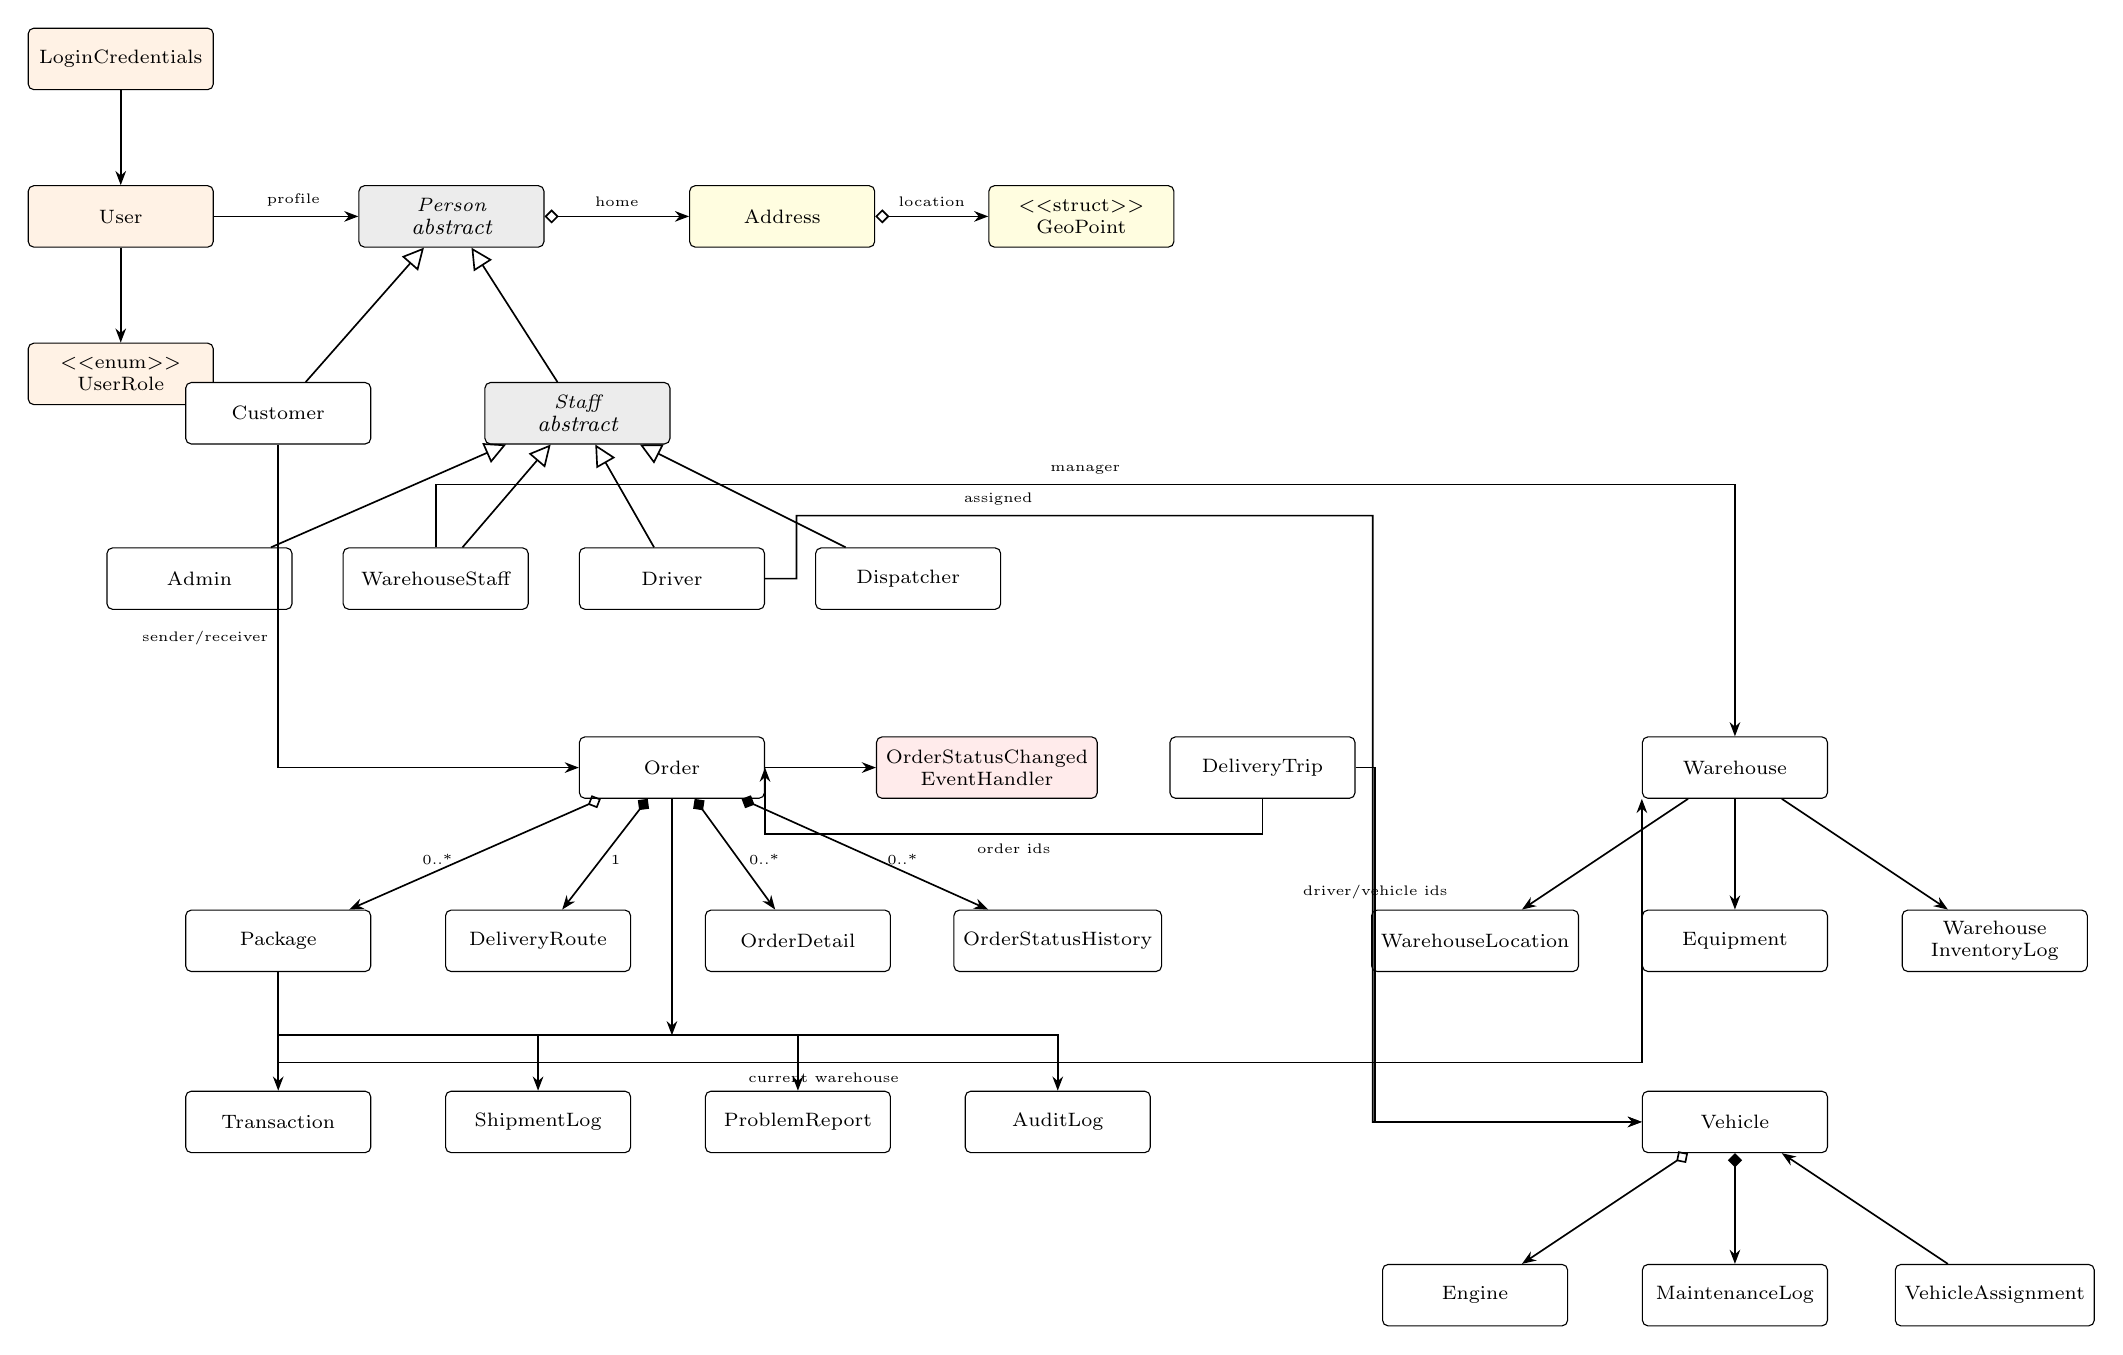
\begin{tikzpicture}[
    font=\scriptsize,
    class/.style={rectangle, draw=black, rounded corners=2pt, align=center, minimum width=2.35cm, minimum height=0.78cm, fill=white},
    abstract/.style={class, fill=gray!15, font=\scriptsize\itshape},
    interface/.style={class, fill=blue!8, minimum width=2.8cm},
    service/.style={class, fill=green!8},
    support/.style={class, fill=orange!10},
    value/.style={class, fill=yellow!12},
    event/.style={class, fill=red!8},
    relation/.style={-{Stealth[length=1.8mm]}, semithick},
    inherit/.style={-{Triangle[open,length=2.7mm,width=2.7mm]}, semithick},
    compose/.style={{Diamond[fill=black,length=1.8mm,width=1.8mm]}-{Stealth[length=1.8mm]}, semithick},
    aggregate/.style={{Diamond[open,length=1.8mm,width=1.8mm]}-{Stealth[length=1.8mm]}, semithick}
]
    % --- ACCOUNT, COMMON TYPES & INTERFACES ---
    \node[support] (LoginCredentials) at (0.0, 15.8) {LoginCredentials};
    \node[support] (User) at (0.0, 13.8) {User};
    \node[support] (UserRole) at (0.0, 11.8) {\textless\textless enum\textgreater\textgreater\\UserRole};

    \node[abstract] (Person) at (4.2, 13.8) {Person\\\footnotesize abstract};
    \node[value] (Address) at (8.4, 13.8) {Address};
    \node[value] (GeoPoint) at (12.2, 13.8) {\textless\textless struct\textgreater\textgreater\\GeoPoint};

    % --- ACTORS ---
    \node[class] (Customer) at (2.0, 11.3) {Customer};
    \node[abstract] (Staff) at (5.8, 11.3) {Staff\\\footnotesize abstract};
    \node[class] (Admin) at (1.0, 9.2) {Admin};
    \node[class] (WarehouseStaff) at (4.0, 9.2) {WarehouseStaff};
    \node[class] (Driver) at (7.0, 9.2) {Driver};
    \node[class] (Dispatcher) at (10.0, 9.2) {Dispatcher};

    % --- ORDER SYSTEM ---
    \node[class] (Order) at (7.0, 6.8) {Order};
    \node[event] (OrderEvent) at (11.0, 6.8) {OrderStatusChanged\\EventHandler};
    \node[class] (Trip) at (14.5, 6.8) {DeliveryTrip};

    \node[class] (Package) at (2.0, 4.6) {Package};
    \node[class] (Route) at (5.3, 4.6) {DeliveryRoute};
    \node[class] (OrderDetail) at (8.6, 4.6) {OrderDetail};
    \node[class] (StatusHistory) at (11.9, 4.6) {OrderStatusHistory};

    \node[class] (Transaction) at (2.0, 2.3) {Transaction};
    \node[class] (ShipmentLog) at (5.3, 2.3) {ShipmentLog};
    \node[class] (ProblemReport) at (8.6, 2.3) {ProblemReport};
    \node[class] (AuditLog) at (11.9, 2.3) {AuditLog};

    % --- WAREHOUSE & VEHICLE SYSTEM ---
    \node[class] (Warehouse) at (20.5, 6.8) {Warehouse};
    \node[class] (WarehouseLocation) at (17.2, 4.6) {WarehouseLocation};
    \node[class] (Equipment) at (20.5, 4.6) {Equipment};
    \node[class] (WarehouseLog) at (23.8, 4.6) {Warehouse\\InventoryLog};

    \node[class] (Vehicle) at (20.5, 2.3) {Vehicle};
    \node[class] (Engine) at (17.2, 0.1) {Engine};
    \node[class] (MaintenanceLog) at (20.5, 0.1) {MaintenanceLog};
    \node[class] (VehicleAssignment) at (23.8, 0.1) {VehicleAssignment};

    % ================= DRAWING RELATIONSHIPS =================

    % Account and common value objects
    \draw[relation] (LoginCredentials) -- (User);
    \draw[relation] (User) -- node[above, pos=0.55] {\tiny profile} (Person);
    \draw[relation] (User) -- (UserRole);
    \draw[aggregate] (Person) -- node[above] {\tiny home} (Address);
    \draw[aggregate] (Address) -- node[above] {\tiny location} (GeoPoint);
    % Inheritances
    \draw[inherit] (Customer) -- (Person);
    \draw[inherit] (Staff) -- (Person);
    \draw[inherit] (Admin) -- (Staff);
    \draw[inherit] (WarehouseStaff) -- (Staff);
    \draw[inherit] (Driver) -- (Staff);
    \draw[inherit] (Dispatcher) -- (Staff);

    % Associations & Aggregations & Compositions
    \draw[relation] (Customer.south) |- node[pos=0.30, left] {\tiny sender/receiver} (Order.west);
    \draw[aggregate] (Order) -- node[left, pos=0.55] {\tiny 0..*} (Package);
    \draw[compose] (Order) -- node[right, pos=0.55] {\tiny 1} (Route);
    \draw[compose] (Order) -- node[right, pos=0.55] {\tiny 0..*} (OrderDetail);
    \draw[compose] (Order) -- node[right, pos=0.55] {\tiny 0..*} (StatusHistory);
    \coordinate (OrderAssocHub) at (7.0, 3.4);
    \draw[relation] (Order.south) -- (OrderAssocHub);
    \draw[relation] (OrderAssocHub) -| (Transaction.north);
    \draw[relation] (OrderAssocHub) -| (ShipmentLog.north);
    \draw[relation] (OrderAssocHub) -| (ProblemReport.north);
    \draw[relation] (OrderAssocHub) -| (AuditLog.north);
    \draw[relation] (Order) -- (OrderEvent);
    \draw[relation] (Trip.south) -- ++(0,-0.45) -| node[pos=0.25, below] {\tiny order ids} (Order.east);
    \draw[relation] (Trip.east) -- ++(0.25,0) |- node[pos=0.20, above] {\tiny driver/vehicle ids} (Vehicle.west);

    \draw[relation] (WarehouseStaff.north) -- ++(0,0.8) -| node[pos=0.25, above] {\tiny manager} (Warehouse.north);
    \draw[relation] (Warehouse) -- (WarehouseLocation);
    \draw[relation] (Warehouse) -- (Equipment);
    \draw[relation] (Warehouse) -- (WarehouseLog);
    \draw[relation] (Package.south) -- ++(0,-1.15) -| node[pos=0.20, below] {\tiny current warehouse} (Warehouse.south west);

    \draw[relation] (Driver.east) -- ++(0.4,0) -- ++(0,0.8) --
        node[above, pos=0.35] {\tiny assigned} (15.9,10.0) -- (15.9,2.3) -- (Vehicle.west);
    \draw[aggregate] (Vehicle) -- (Engine);
    \draw[compose] (Vehicle) -- (MaintenanceLog);
    \draw[relation] (VehicleAssignment) -- (Vehicle);

\end{tikzpicture}
}
\caption{Sơ đồ lớp tổng quát của hệ thống Logistics}
\end{figure}

\begin{table}[H]
\centering
\small
\begin{tabular}{p{3.2cm}p{4.0cm}p{6.7cm}}
\toprule
\textbf{Lớp} & \textbf{Trường định danh \{id\}} & \textbf{Trường tham chiếu \{ref\}} \\
\midrule
\texttt{Person} & \texttt{Id} & \texttt{HomeAddress} tham chiếu đối tượng \texttt{Address}. \\
\texttt{User} & \texttt{UserId}, \texttt{Username} & \texttt{Person} liên kết hồ sơ tác nhân. \\
\texttt{Staff} & \texttt{StaffID} & \texttt{AccountID} liên kết tài khoản. \\
\texttt{Order} & \texttt{TrackingNumber} & \texttt{SenderID}, \texttt{ReceiverID}, \texttt{AssignedDriverID}, \texttt{AssignedVehicleID}. \\
\texttt{Package} & \texttt{PackageID} & \texttt{OrderID}, \texttt{CurrentWarehouseID}. \\
\texttt{DeliveryTrip} & \texttt{TripID} & \texttt{DriverID}, \texttt{VehicleID}, \texttt{OrderIds}. \\
\texttt{Transaction} & \texttt{TransactionID} & \texttt{OrderID}. \\
\texttt{ProblemReport} & \texttt{ReportID} & \texttt{OrderID}. \\
\texttt{ShipmentLog} & \texttt{LogID} & \texttt{TrackingNumber}. \\
\texttt{AuditLog} & \texttt{AuditLogId} & \texttt{ActorUsername}, \texttt{EntityType}, \texttt{EntityId}. \\
\texttt{Vehicle} & \texttt{VehicleID} & \texttt{AllowedDrivers}, \texttt{MaintenanceHistory}, \texttt{VehicleEngine}. \\
\texttt{Warehouse} & \texttt{WarehouseID} & \texttt{Manager}. \\
\texttt{WarehouseLocation} & \texttt{LocationID} & \texttt{WarehouseID}. \\
\texttt{WarehouseInventoryLog} & \texttt{LogID} & \texttt{WarehouseID}, \texttt{PackageID}, \texttt{TrackingNumber}. \\
\texttt{Equipment} & \texttt{EquipmentID} & \texttt{WarehouseID}. \\
\texttt{VehicleAssignment} & \texttt{AssignmentID} & \texttt{DriverID}, \texttt{VehicleID}. \\
\bottomrule
\end{tabular}
\caption{Các trường định danh và tham chiếu chính trong domain model}
\end{table}

\begin{figure}[H]
\centering
\resizebox{\textwidth}{!}{
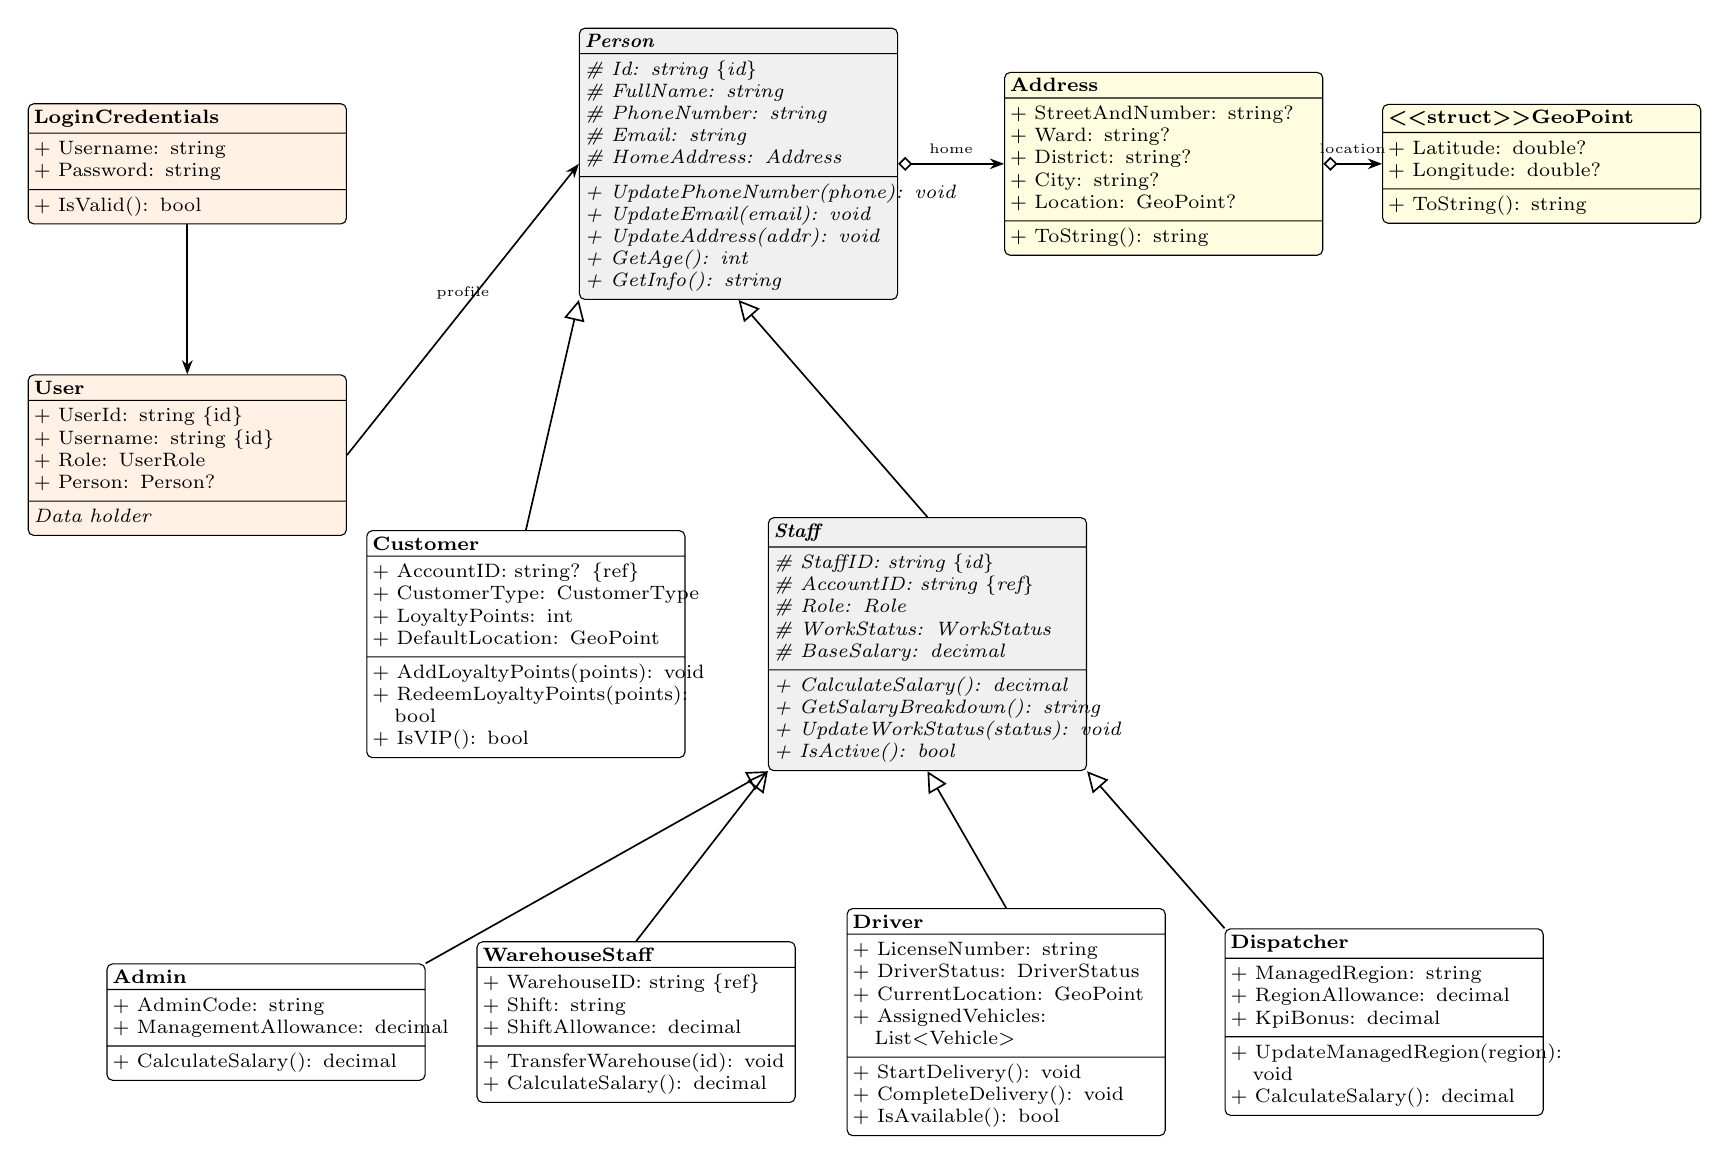
\begin{tikzpicture}[
    font=\scriptsize,
    uml/.style={rectangle split, rectangle split parts=3, rectangle split part align={center,left,left}, draw=black, rounded corners=2pt, text width=3.9cm, inner sep=2pt, fill=white},
    umlabstract/.style={uml, fill=gray!12, font=\scriptsize\itshape},
    umlsupport/.style={uml, fill=orange!10},
    umlvalue/.style={uml, fill=yellow!12},
    inherit/.style={-{Triangle[open,length=2.6mm,width=2.6mm]}, semithick},
    relation/.style={-{Stealth[length=1.8mm]}, semithick},
    aggregate/.style={{Diamond[open,length=1.8mm,width=1.8mm]}-{Stealth[length=1.8mm]}, semithick}
]
\node[umlsupport] (Credentials) at (-1.8,8.3) {\textbf{LoginCredentials}
\nodepart{second}
\begin{tabular}{@{}l@{}}
+ Username: string\\
+ Password: string
\end{tabular}
\nodepart{third}
\begin{tabular}{@{}l@{}}
+ IsValid(): bool
\end{tabular}};

\node[umlsupport] (User) at (-1.8,4.6) {\textbf{User}
\nodepart{second}
\begin{tabular}{@{}l@{}}
+ UserId: string \{id\}\\
+ Username: string \{id\}\\
+ Role: UserRole\\
+ Person: Person?
\end{tabular}
\nodepart{third}
\begin{tabular}{@{}l@{}}
\textit{Data holder}
\end{tabular}};

\node[umlabstract] (Person) at (5.2,8.3) {\textbf{Person}
\nodepart{second}
\begin{tabular}{@{}l@{}}
\# Id: string \{id\}\\
\# FullName: string\\
\# PhoneNumber: string\\
\# Email: string\\
\# HomeAddress: Address
\end{tabular}
\nodepart{third}
\begin{tabular}{@{}l@{}}
+ UpdatePhoneNumber(phone): void\\
+ UpdateEmail(email): void\\
+ UpdateAddress(addr): void\\
+ GetAge(): int\\
+ GetInfo(): string
\end{tabular}};

\node[umlvalue] (Address) at (10.6,8.3) {\textbf{Address}
\nodepart{second}
\begin{tabular}{@{}l@{}}
+ StreetAndNumber: string?\\
+ Ward: string?\\
+ District: string?\\
+ City: string?\\
+ Location: GeoPoint?
\end{tabular}
\nodepart{third}
\begin{tabular}{@{}l@{}}
+ ToString(): string
\end{tabular}};

\node[umlvalue] (GeoPoint) at (15.4,8.3) {\textbf{\textless\textless struct\textgreater\textgreater GeoPoint}
\nodepart{second}
\begin{tabular}{@{}l@{}}
+ Latitude: double?\\
+ Longitude: double?
\end{tabular}
\nodepart{third}
\begin{tabular}{@{}l@{}}
+ ToString(): string
\end{tabular}};

\node[uml] (Customer) at (2.5,2.2) {\textbf{Customer}
\nodepart{second}
\begin{tabular}{@{}l@{}}
+ AccountID: string? \{ref\}\\
+ CustomerType: CustomerType\\
+ LoyaltyPoints: int\\
+ DefaultLocation: GeoPoint
\end{tabular}
\nodepart{third}
\begin{tabular}{@{}l@{}}
+ AddLoyaltyPoints(points): void\\
+ RedeemLoyaltyPoints(points):\\
\quad bool\\
+ IsVIP(): bool
\end{tabular}};

\node[umlabstract] (Staff) at (7.6,2.2) {\textbf{Staff}
\nodepart{second}
\begin{tabular}{@{}l@{}}
\# StaffID: string \{id\}\\
\# AccountID: string \{ref\}\\
\# Role: Role\\
\# WorkStatus: WorkStatus\\
\# BaseSalary: decimal
\end{tabular}
\nodepart{third}
\begin{tabular}{@{}l@{}}
+ CalculateSalary(): decimal\\
+ GetSalaryBreakdown(): string\\
+ UpdateWorkStatus(status): void\\
+ IsActive(): bool
\end{tabular}};

\node[uml] (Admin) at (-0.8,-2.6) {\textbf{Admin}
\nodepart{second}
\begin{tabular}{@{}l@{}}
+ AdminCode: string\\
+ ManagementAllowance: decimal
\end{tabular}
\nodepart{third}
\begin{tabular}{@{}l@{}}
+ CalculateSalary(): decimal
\end{tabular}};

\node[uml] (WarehouseStaff) at (3.9,-2.6) {\textbf{WarehouseStaff}
\nodepart{second}
\begin{tabular}{@{}l@{}}
+ WarehouseID: string \{ref\}\\
+ Shift: string\\
+ ShiftAllowance: decimal
\end{tabular}
\nodepart{third}
\begin{tabular}{@{}l@{}}
+ TransferWarehouse(id): void\\
+ CalculateSalary(): decimal
\end{tabular}};

\node[uml] (Driver) at (8.6,-2.6) {\textbf{Driver}
\nodepart{second}
\begin{tabular}{@{}l@{}}
+ LicenseNumber: string\\
+ DriverStatus: DriverStatus\\
+ CurrentLocation: GeoPoint\\
+ AssignedVehicles:\\
\quad List\textless Vehicle\textgreater
\end{tabular}
\nodepart{third}
\begin{tabular}{@{}l@{}}
+ StartDelivery(): void\\
+ CompleteDelivery(): void\\
+ IsAvailable(): bool
\end{tabular}};

\node[uml] (Dispatcher) at (13.4,-2.6) {\textbf{Dispatcher}
\nodepart{second}
\begin{tabular}{@{}l@{}}
+ ManagedRegion: string\\
+ RegionAllowance: decimal\\
+ KpiBonus: decimal
\end{tabular}
\nodepart{third}
\begin{tabular}{@{}l@{}}
+ UpdateManagedRegion(region):\\
\quad void\\
+ CalculateSalary(): decimal
\end{tabular}};

\draw[relation] (Credentials.south) -- (User.north);
\draw[relation] (User.east) -- node[above] {\tiny profile} (Person.west);
\draw[aggregate] (Person) -- node[above] {\tiny home} (Address);
\draw[aggregate] (Address) -- node[above] {\tiny location} (GeoPoint);
\draw[inherit] (Customer.north) -- (Person.south west);
\draw[inherit] (Staff.north) -- (Person.south);
\draw[inherit] (Admin.north east) -- (Staff.south west);
\draw[inherit] (WarehouseStaff.north) -- (Staff.south west);
\draw[inherit] (Driver.north) -- (Staff.south);
\draw[inherit] (Dispatcher.north west) -- (Staff.south east);
\end{tikzpicture}
}
\caption{Sơ đồ lớp chi tiết nhóm tác nhân, tài khoản và kiểu giá trị dùng chung}
\end{figure}

\begin{figure}[H]
\centering
\resizebox{\textwidth}{!}{
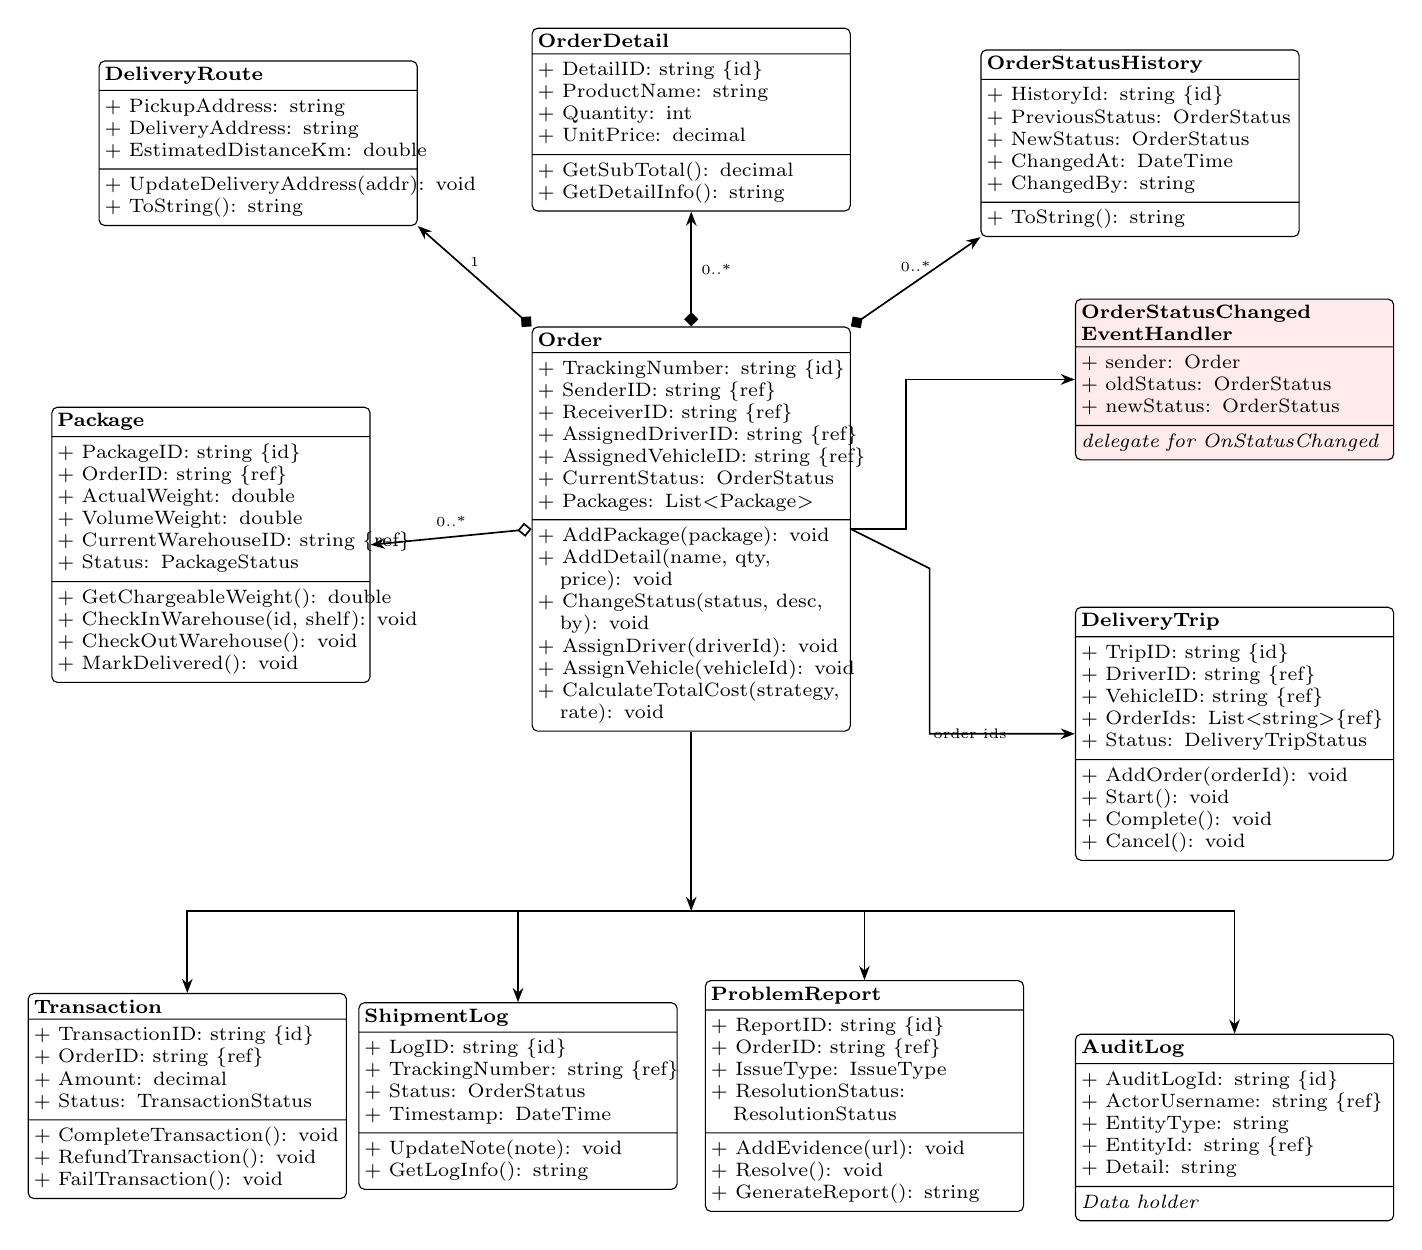
\begin{tikzpicture}[
    font=\scriptsize,
    uml/.style={rectangle split, rectangle split parts=3, rectangle split part align={center,left,left}, draw=black, rounded corners=2pt, text width=3.9cm, inner sep=2pt, fill=white},
    umlevent/.style={uml, fill=red!8},
    inherit/.style={-{Triangle[open,length=2.6mm,width=2.6mm]}, semithick},
    relation/.style={-{Stealth[length=1.8mm]}, semithick},
    compose/.style={{Diamond[fill=black,length=1.8mm,width=1.8mm]}-{Stealth[length=1.8mm]}, semithick},
    aggregate/.style={{Diamond[open,length=1.8mm,width=1.8mm]}-{Stealth[length=1.8mm]}, semithick}
]
\node[uml] (Order) at (7.2,6.2) {\textbf{Order}
\nodepart{second}
\begin{tabular}{@{}l@{}}
+ TrackingNumber: string \{id\}\\
+ SenderID: string \{ref\}\\
+ ReceiverID: string \{ref\}\\
+ AssignedDriverID: string \{ref\}\\
+ AssignedVehicleID: string \{ref\}\\
+ CurrentStatus: OrderStatus\\
+ Packages: List\textless Package\textgreater
\end{tabular}
\nodepart{third}
\begin{tabular}{@{}l@{}}
+ AddPackage(package): void\\
+ AddDetail(name, qty,\\
\quad price): void\\
+ ChangeStatus(status, desc,\\
\quad by): void\\
+ AssignDriver(driverId): void\\
+ AssignVehicle(vehicleId): void\\
+ CalculateTotalCost(strategy,\\
\quad rate): void
\end{tabular}};

\node[uml] (Route) at (1.7,11.1) {\textbf{DeliveryRoute}
\nodepart{second}
\begin{tabular}{@{}l@{}}
+ PickupAddress: string\\
+ DeliveryAddress: string\\
+ EstimatedDistanceKm: double
\end{tabular}
\nodepart{third}
\begin{tabular}{@{}l@{}}
+ UpdateDeliveryAddress(addr): void\\
+ ToString(): string
\end{tabular}};

\node[uml] (Detail) at (7.2,11.4) {\textbf{OrderDetail}
\nodepart{second}
\begin{tabular}{@{}l@{}}
+ DetailID: string \{id\}\\
+ ProductName: string\\
+ Quantity: int\\
+ UnitPrice: decimal
\end{tabular}
\nodepart{third}
\begin{tabular}{@{}l@{}}
+ GetSubTotal(): decimal\\
+ GetDetailInfo(): string
\end{tabular}};

\node[uml] (History) at (12.9,11.1) {\textbf{OrderStatusHistory}
\nodepart{second}
\begin{tabular}{@{}l@{}}
+ HistoryId: string \{id\}\\
+ PreviousStatus: OrderStatus\\
+ NewStatus: OrderStatus\\
+ ChangedAt: DateTime\\
+ ChangedBy: string
\end{tabular}
\nodepart{third}
\begin{tabular}{@{}l@{}}
+ ToString(): string
\end{tabular}};

\node[uml] (Package) at (1.1,6.0) {\textbf{Package}
\nodepart{second}
\begin{tabular}{@{}l@{}}
+ PackageID: string \{id\}\\
+ OrderID: string \{ref\}\\
+ ActualWeight: double\\
+ VolumeWeight: double\\
+ CurrentWarehouseID: string \{ref\}\\
+ Status: PackageStatus
\end{tabular}
\nodepart{third}
\begin{tabular}{@{}l@{}}
+ GetChargeableWeight(): double\\
+ CheckInWarehouse(id, shelf): void\\
+ CheckOutWarehouse(): void\\
+ MarkDelivered(): void
\end{tabular}};

\node[umlevent] (Event) at (14.1,8.1) {\textbf{OrderStatusChanged\\EventHandler}
\nodepart{second}
\begin{tabular}{@{}l@{}}
+ sender: Order\\
+ oldStatus: OrderStatus\\
+ newStatus: OrderStatus
\end{tabular}
\nodepart{third}
\begin{tabular}{@{}l@{}}
\textit{delegate for OnStatusChanged}
\end{tabular}};

\node[uml] (Trip) at (14.1,3.6) {\textbf{DeliveryTrip}
\nodepart{second}
\begin{tabular}{@{}l@{}}
+ TripID: string \{id\}\\
+ DriverID: string \{ref\}\\
+ VehicleID: string \{ref\}\\
+ OrderIds: List\textless string\textgreater \{ref\}\\
+ Status: DeliveryTripStatus
\end{tabular}
\nodepart{third}
\begin{tabular}{@{}l@{}}
+ AddOrder(orderId): void\\
+ Start(): void\\
+ Complete(): void\\
+ Cancel(): void
\end{tabular}};

\node[uml] (Transaction) at (0.8,-1.0) {\textbf{Transaction}
\nodepart{second}
\begin{tabular}{@{}l@{}}
+ TransactionID: string \{id\}\\
+ OrderID: string \{ref\}\\
+ Amount: decimal\\
+ Status: TransactionStatus
\end{tabular}
\nodepart{third}
\begin{tabular}{@{}l@{}}
+ CompleteTransaction(): void\\
+ RefundTransaction(): void\\
+ FailTransaction(): void
\end{tabular}};

\node[uml] (ShipmentLog) at (5.0,-1.0) {\textbf{ShipmentLog}
\nodepart{second}
\begin{tabular}{@{}l@{}}
+ LogID: string \{id\}\\
+ TrackingNumber: string \{ref\}\\
+ Status: OrderStatus\\
+ Timestamp: DateTime
\end{tabular}
\nodepart{third}
\begin{tabular}{@{}l@{}}
+ UpdateNote(note): void\\
+ GetLogInfo(): string
\end{tabular}};

\node[uml] (ProblemReport) at (9.4,-1.0) {\textbf{ProblemReport}
\nodepart{second}
\begin{tabular}{@{}l@{}}
+ ReportID: string \{id\}\\
+ OrderID: string \{ref\}\\
+ IssueType: IssueType\\
+ ResolutionStatus:\\
\quad ResolutionStatus
\end{tabular}
\nodepart{third}
\begin{tabular}{@{}l@{}}
+ AddEvidence(url): void\\
+ Resolve(): void\\
+ GenerateReport(): string
\end{tabular}};

\node[uml] (AuditLog) at (14.1,-1.4) {\textbf{AuditLog}
\nodepart{second}
\begin{tabular}{@{}l@{}}
+ AuditLogId: string \{id\}\\
+ ActorUsername: string \{ref\}\\
+ EntityType: string\\
+ EntityId: string \{ref\}\\
+ Detail: string
\end{tabular}
\nodepart{third}
\begin{tabular}{@{}l@{}}
\textit{Data holder}
\end{tabular}};

\draw[compose] (Order.north west) -- node[above] {\tiny 1} (Route.south east);
\draw[compose] (Order.north) -- node[right] {\tiny 0..*} (Detail.south);
\draw[compose] (Order.north east) -- node[above] {\tiny 0..*} (History.south west);
\draw[aggregate] (Order.west) -- node[above] {\tiny 0..*} (Package.east);
\draw[relation] (Order.east) -- ++(0.7,0) |- (Event.west);
\draw[relation] (Order.east) -- ++(1.0,-0.5) |- node[pos=0.80,left] {\tiny order ids} (Trip.west);
\coordinate (OrderRefs) at (7.2,1.35);
\draw[relation] (Order.south) -- (OrderRefs);
\draw[relation] (OrderRefs) -| (Transaction.north);
\draw[relation] (OrderRefs) -| (ShipmentLog.north);
\draw[relation] (OrderRefs) -| (ProblemReport.north);
\draw[relation] (OrderRefs) -| (AuditLog.north);
\end{tikzpicture}
}
\caption{Sơ đồ lớp chi tiết nhóm đơn hàng và nghiệp vụ vận chuyển}
\end{figure}

\begin{figure}[H]
\centering
\resizebox{\textwidth}{!}{
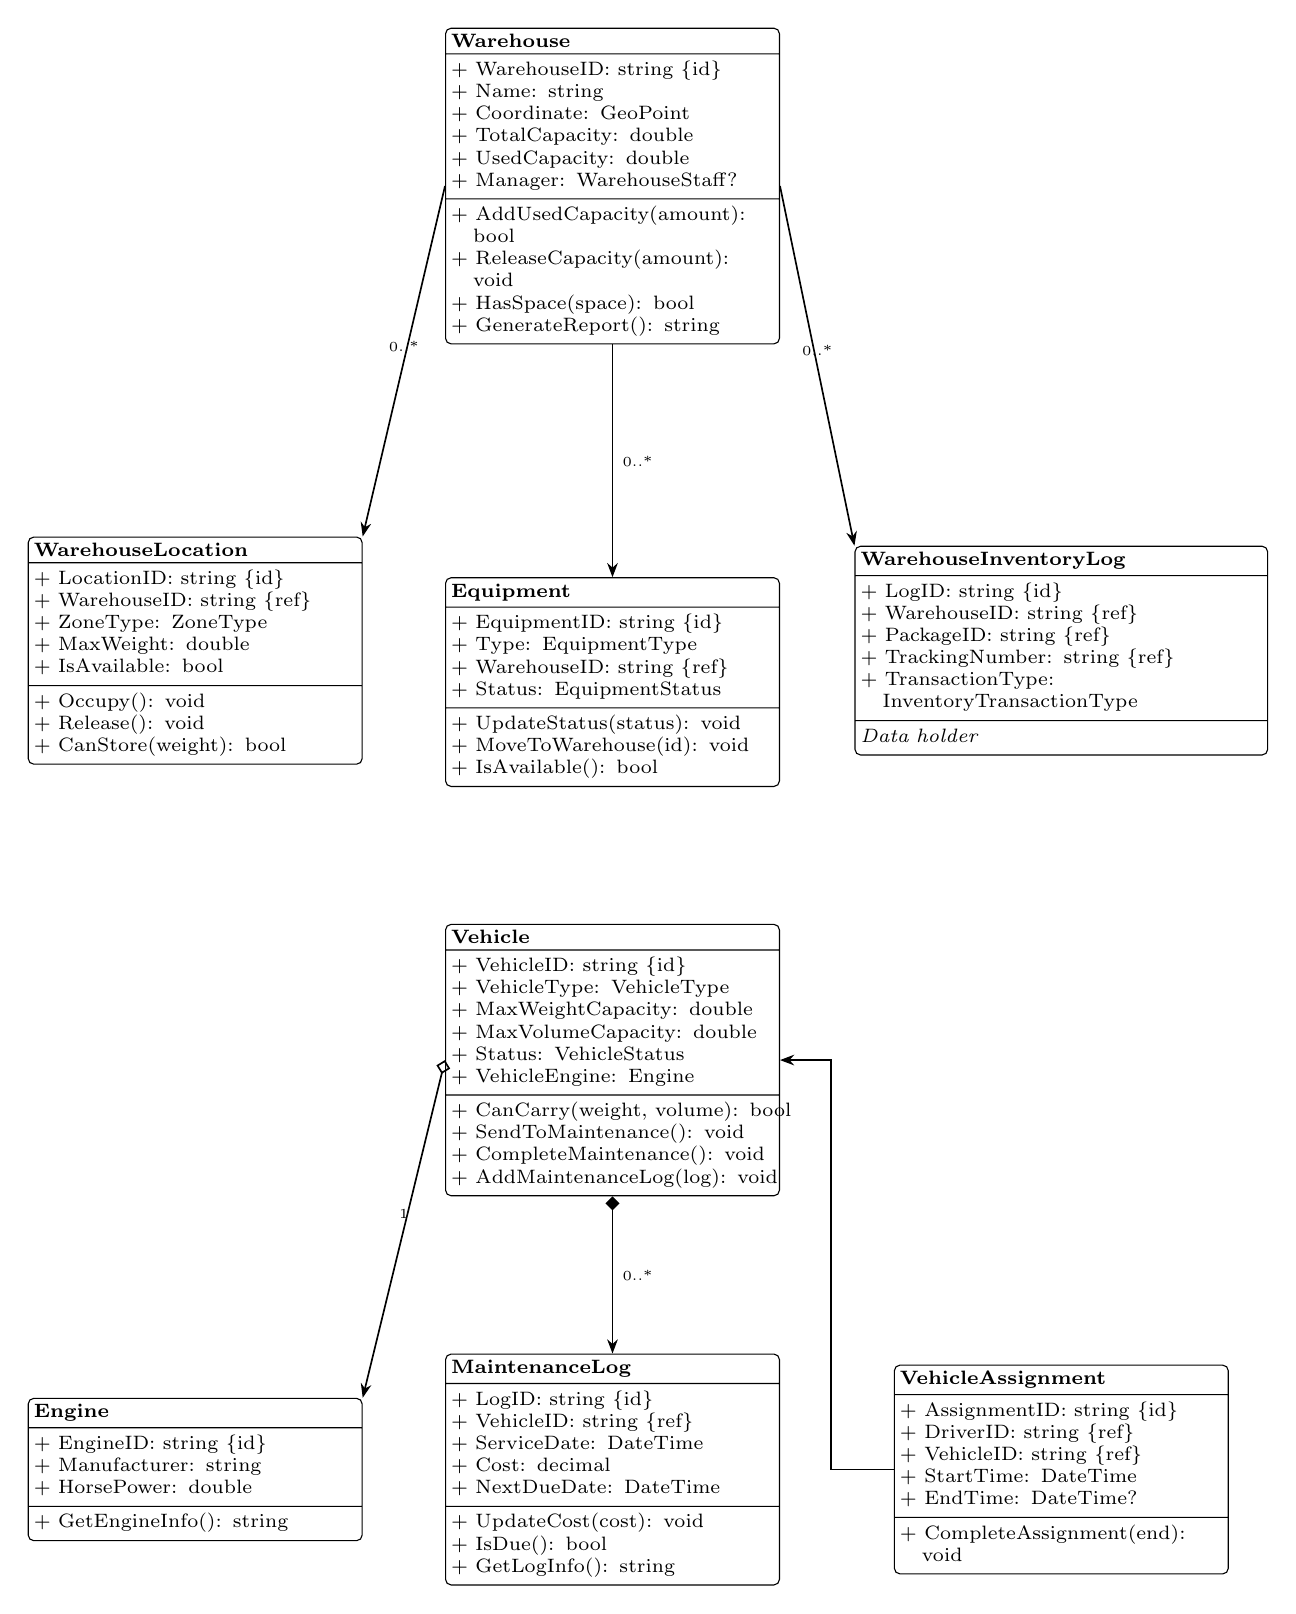
\begin{tikzpicture}[
    font=\scriptsize,
    uml/.style={rectangle split, rectangle split parts=3, rectangle split part align={center,left,left}, draw=black, rounded corners=2pt, text width=4.1cm, inner sep=2pt, fill=white},
    umlwide/.style={uml, text width=5.1cm},
    relation/.style={-{Stealth[length=1.8mm]}, semithick},
    compose/.style={{Diamond[fill=black,length=1.8mm,width=1.8mm]}-{Stealth[length=1.8mm]}, semithick},
    aggregate/.style={{Diamond[open,length=1.8mm,width=1.8mm]}-{Stealth[length=1.8mm]}, semithick}
]
\node[uml] (Warehouse) at (5.8,11.3) {\textbf{Warehouse}
\nodepart{second}
\begin{tabular}{@{}l@{}}
+ WarehouseID: string \{id\}\\
+ Name: string\\
+ Coordinate: GeoPoint\\
+ TotalCapacity: double\\
+ UsedCapacity: double\\
+ Manager: WarehouseStaff?
\end{tabular}
\nodepart{third}
\begin{tabular}{@{}l@{}}
+ AddUsedCapacity(amount):\\
\quad bool\\
+ ReleaseCapacity(amount):\\
\quad void\\
+ HasSpace(space): bool\\
+ GenerateReport(): string
\end{tabular}};

\node[uml] (Location) at (0.5,5.4) {\textbf{WarehouseLocation}
\nodepart{second}
\begin{tabular}{@{}l@{}}
+ LocationID: string \{id\}\\
+ WarehouseID: string \{ref\}\\
+ ZoneType: ZoneType\\
+ MaxWeight: double\\
+ IsAvailable: bool
\end{tabular}
\nodepart{third}
\begin{tabular}{@{}l@{}}
+ Occupy(): void\\
+ Release(): void\\
+ CanStore(weight): bool
\end{tabular}};

\node[uml] (Equipment) at (5.8,5.0) {\textbf{Equipment}
\nodepart{second}
\begin{tabular}{@{}l@{}}
+ EquipmentID: string \{id\}\\
+ Type: EquipmentType\\
+ WarehouseID: string \{ref\}\\
+ Status: EquipmentStatus
\end{tabular}
\nodepart{third}
\begin{tabular}{@{}l@{}}
+ UpdateStatus(status): void\\
+ MoveToWarehouse(id): void\\
+ IsAvailable(): bool
\end{tabular}};

\node[umlwide] (WarehouseLog) at (11.5,5.4) {\textbf{WarehouseInventoryLog}
\nodepart{second}
\begin{tabular}{@{}l@{}}
+ LogID: string \{id\}\\
+ WarehouseID: string \{ref\}\\
+ PackageID: string \{ref\}\\
+ TrackingNumber: string \{ref\}\\
+ TransactionType:\\
\quad InventoryTransactionType
\end{tabular}
\nodepart{third}
\begin{tabular}{@{}l@{}}
\textit{Data holder}
\end{tabular}};

\node[uml] (Vehicle) at (5.8,0.2) {\textbf{Vehicle}
\nodepart{second}
\begin{tabular}{@{}l@{}}
+ VehicleID: string \{id\}\\
+ VehicleType: VehicleType\\
+ MaxWeightCapacity: double\\
+ MaxVolumeCapacity: double\\
+ Status: VehicleStatus\\
+ VehicleEngine: Engine
\end{tabular}
\nodepart{third}
\begin{tabular}{@{}l@{}}
+ CanCarry(weight, volume): bool\\
+ SendToMaintenance(): void\\
+ CompleteMaintenance(): void\\
+ AddMaintenanceLog(log): void
\end{tabular}};

\node[uml] (Engine) at (0.5,-5.0) {\textbf{Engine}
\nodepart{second}
\begin{tabular}{@{}l@{}}
+ EngineID: string \{id\}\\
+ Manufacturer: string\\
+ HorsePower: double
\end{tabular}
\nodepart{third}
\begin{tabular}{@{}l@{}}
+ GetEngineInfo(): string
\end{tabular}};

\node[uml] (Maintenance) at (5.8,-5.0) {\textbf{MaintenanceLog}
\nodepart{second}
\begin{tabular}{@{}l@{}}
+ LogID: string \{id\}\\
+ VehicleID: string \{ref\}\\
+ ServiceDate: DateTime\\
+ Cost: decimal\\
+ NextDueDate: DateTime
\end{tabular}
\nodepart{third}
\begin{tabular}{@{}l@{}}
+ UpdateCost(cost): void\\
+ IsDue(): bool\\
+ GetLogInfo(): string
\end{tabular}};

\node[uml] (Assignment) at (11.5,-5.0) {\textbf{VehicleAssignment}
\nodepart{second}
\begin{tabular}{@{}l@{}}
+ AssignmentID: string \{id\}\\
+ DriverID: string \{ref\}\\
+ VehicleID: string \{ref\}\\
+ StartTime: DateTime\\
+ EndTime: DateTime?
\end{tabular}
\nodepart{third}
\begin{tabular}{@{}l@{}}
+ CompleteAssignment(end):\\
\quad void
\end{tabular}};

\draw[relation] (Warehouse.west) -- node[above] {\tiny 0..*} (Location.north east);
\draw[relation] (Warehouse.south) -- node[right] {\tiny 0..*} (Equipment.north);
\draw[relation] (Warehouse.east) -- node[above] {\tiny 0..*} (WarehouseLog.north west);
\draw[aggregate] (Vehicle.west) -- node[above] {\tiny 1} (Engine.north east);
\draw[compose] (Vehicle.south) -- node[right] {\tiny 0..*} (Maintenance.north);
\draw[relation] (Assignment.west) -- ++(-0.8,0) |- (Vehicle.east);
\end{tikzpicture}
}
\caption{Sơ đồ lớp chi tiết nhóm kho, phương tiện và hạ tầng logistics}
\end{figure}

\begin{figure}[H]
\centering
\resizebox{0.88\textwidth}{!}{
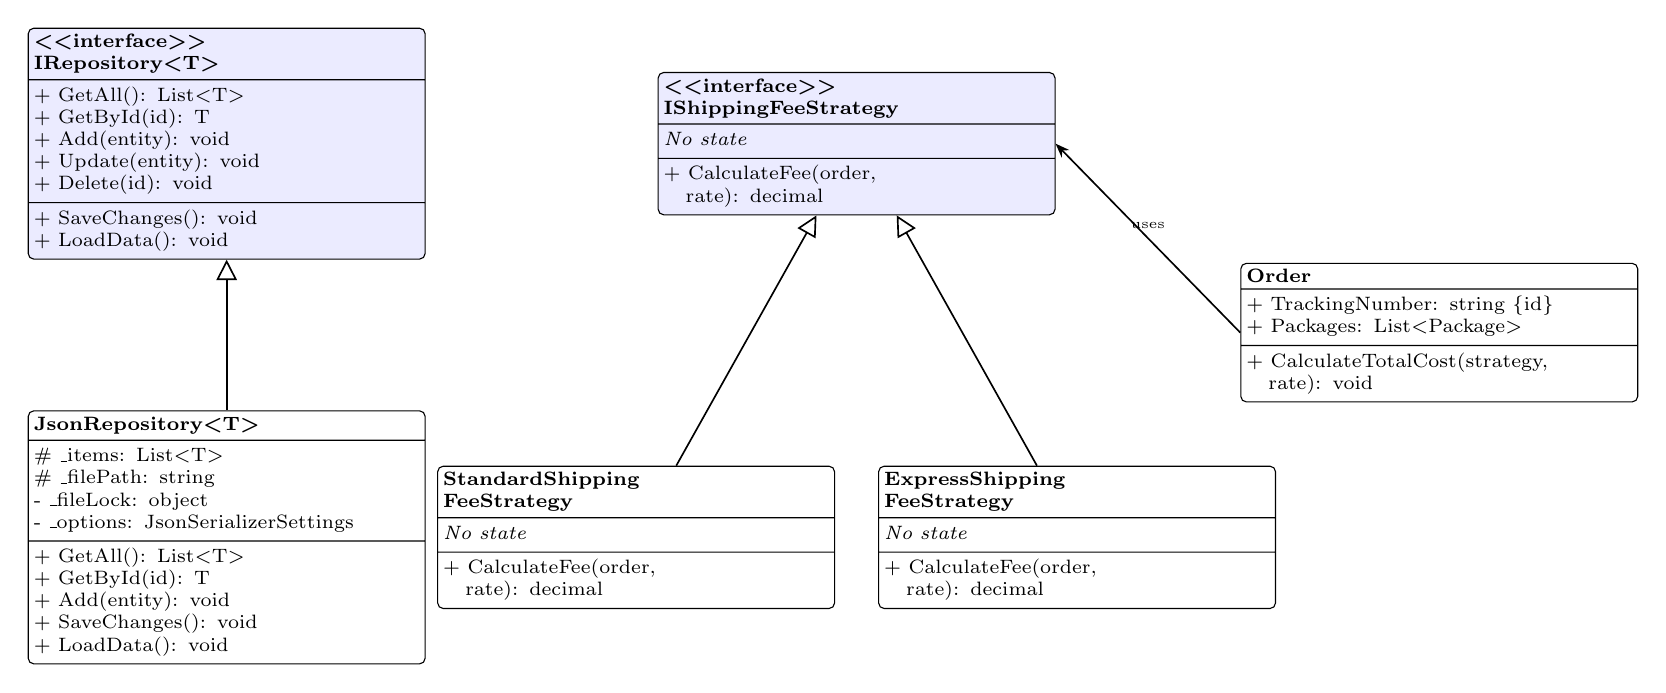
\begin{tikzpicture}[
    font=\scriptsize,
    uml/.style={rectangle split, rectangle split parts=3, rectangle split part align={center,left,left}, draw=black, rounded corners=2pt, text width=4.9cm, inner sep=2pt, fill=white},
    umlinterface/.style={uml, fill=blue!8},
    impl/.style={-{Triangle[open,length=2.6mm,width=2.6mm]}, semithick},
    relation/.style={-{Stealth[length=1.8mm]}, semithick}
]
\node[umlinterface] (Repo) at (0,4.4) {\textbf{\textless\textless interface\textgreater\textgreater\\IRepository\textless T\textgreater}
\nodepart{second}
\begin{tabular}{@{}l@{}}
+ GetAll(): List\textless T\textgreater\\
+ GetById(id): T\\
+ Add(entity): void\\
+ Update(entity): void\\
+ Delete(id): void
\end{tabular}
\nodepart{third}
\begin{tabular}{@{}l@{}}
+ SaveChanges(): void\\
+ LoadData(): void
\end{tabular}};

\node[uml] (JsonRepo) at (0,-0.6) {\textbf{JsonRepository\textless T\textgreater}
\nodepart{second}
\begin{tabular}{@{}l@{}}
\# \_items: List\textless T\textgreater\\
\# \_filePath: string\\
- \_fileLock: object\\
- \_options: JsonSerializerSettings
\end{tabular}
\nodepart{third}
\begin{tabular}{@{}l@{}}
+ GetAll(): List\textless T\textgreater\\
+ GetById(id): T\\
+ Add(entity): void\\
+ SaveChanges(): void\\
+ LoadData(): void
\end{tabular}};

\node[umlinterface] (Strategy) at (8.0,4.4) {\textbf{\textless\textless interface\textgreater\textgreater\\IShippingFeeStrategy}
\nodepart{second}
\begin{tabular}{@{}l@{}}
\textit{No state}
\end{tabular}
\nodepart{third}
\begin{tabular}{@{}l@{}}
+ CalculateFee(order,\\
\quad rate): decimal
\end{tabular}};

\node[uml] (Standard) at (5.2,-0.6) {\textbf{StandardShipping\\FeeStrategy}
\nodepart{second}
\begin{tabular}{@{}l@{}}
\textit{No state}
\end{tabular}
\nodepart{third}
\begin{tabular}{@{}l@{}}
+ CalculateFee(order,\\
\quad rate): decimal
\end{tabular}};

\node[uml] (Express) at (10.8,-0.6) {\textbf{ExpressShipping\\FeeStrategy}
\nodepart{second}
\begin{tabular}{@{}l@{}}
\textit{No state}
\end{tabular}
\nodepart{third}
\begin{tabular}{@{}l@{}}
+ CalculateFee(order,\\
\quad rate): decimal
\end{tabular}};

\node[uml] (OrderRef) at (15.4,2.0) {\textbf{Order}
\nodepart{second}
\begin{tabular}{@{}l@{}}
+ TrackingNumber: string \{id\}\\
+ Packages: List\textless Package\textgreater
\end{tabular}
\nodepart{third}
\begin{tabular}{@{}l@{}}
+ CalculateTotalCost(strategy,\\
\quad rate): void
\end{tabular}};

\draw[impl] (JsonRepo) -- (Repo);
\draw[impl] (Standard) -- (Strategy);
\draw[impl] (Express) -- (Strategy);
\draw[relation] (OrderRef.west) -- node[above] {\tiny uses} (Strategy.east);
\end{tikzpicture}
}
\caption{Sơ đồ lớp chi tiết cho Repository Pattern và Strategy Pattern}
\end{figure}

\subsubsection{Các tính chất cơ bản của Lập trình hướng đối tượng (OOP)}

Dự án Logistics được thiết kế dựa trên các nguyên lý lập trình hướng đối tượng nền tảng, giúp hệ thống đạt tính bền vững, dễ bảo trì và khả năng mở rộng tốt. Dưới đây là phân tích chi tiết cách áp dụng bốn trụ cột OOP cùng các ví dụ cụ thể từ mã nguồn.

\subsubsection*{a. Tính đóng gói (Encapsulation)}

Tính đóng gói được thể hiện qua việc che giấu trạng thái nội tại của đối tượng và chỉ cho phép thay đổi dữ liệu thông qua các phương thức công khai (API nghiệp vụ). Các thuộc tính quan trọng trong các lớp thực thể (như \texttt{Order}, \texttt{Package}, \texttt{Vehicle}) đều được khai báo với setter có phạm vi truy cập hạn chế (\texttt{private set} hoặc \texttt{protected set}). Điều này ngăn chặn việc gán giá trị tùy tiện từ bên ngoài lớp, bảo vệ tính toàn vẹn dữ liệu.

Ví dụ, trạng thái của đơn hàng (\texttt{OrderStatus}) và lịch sử thay đổi trạng thái (\texttt{StatusHistories}) không thể chỉnh sửa trực tiếp. Muốn cập nhật trạng thái đơn hàng, đối tượng bên ngoài phải gọi phương thức \texttt{ChangeStatus()}. Phương thức này chịu trách nhiệm:
\begin{enumerate}[label=\arabic*.]
    \item Kiểm tra tính hợp lệ của luồng chuyển đổi trạng thái thông qua hàm kiểm thử tĩnh \texttt{CanTransition()}.
    \item Ghi nhận lịch sử thay đổi trạng thái vào danh sách tự quản lý (quan hệ Composition).
    \item Đồng bộ hóa trạng thái của tất cả các gói hàng thuộc đơn hàng đó (quan hệ Aggregation).
    \item Kích hoạt sự kiện \texttt{OnStatusChanged} để thông báo cho các hệ thống quan sát khác (Observer Pattern).
\end{enumerate}

\begin{listing}[H]
\caption{Phương thức ChangeStatus thể hiện tính đóng gói trong lớp Order}
\begin{minted}{csharp}
public void ChangeStatus(OrderStatus newStatus, string description = "", string changedBy = "System")
{
    // Kiểm tra ràng buộc chuyển đổi trạng thái trước khi thay đổi
    if (!CanTransitionTo(newStatus))
    {
        throw new InvalidOrderException($"Khong the chuyen trang thai tu {CurrentStatus} sang {newStatus}");
    }

    if (CurrentStatus != newStatus)
    {
        OrderStatus oldStatus = CurrentStatus;
        
        // Tạo lịch sử thay đổi trạng thái (Composition)
        OrderStatusHistory historyItem = new OrderStatusHistory
        {
            PreviousStatus = oldStatus,
            NewStatus = newStatus,
            ChangedAt = DateTime.Now,
            Location = this.Route != null ? this.Route.ToString() : "Unknown",
            Description = description,
            ChangedBy = changedBy
        };
        StatusHistories.Add(historyItem);
        
        // Thực hiện cập nhật trạng thái
        CurrentStatus = newStatus;
        
        // Đồng bộ trạng thái các kiện hàng con
        SynchronizePackageStatuses(oldStatus, newStatus);
        
        // Phát sự kiện thông báo (Observer)
        OnStatusChanged?.Invoke(this, oldStatus, newStatus);
    }
}
\end{minted}
\end{listing}

Tương tự, lớp \texttt{Package} đóng gói trạng thái vị trí kho của nó. Thuộc tính \texttt{CurrentWarehouseID} và \texttt{CurrentShelfLocation} chỉ được cập nhật qua phương thức nghiệp vụ \texttt{CheckInWarehouse()}, bảo đảm rằng khi kiện hàng nằm trong kho thì thông tin vị trí kệ kệ cũng được cập nhật đồng thời một cách an toàn.

\subsubsection*{b. Tính trừu tượng (Abstraction)}

Tính trừu tượng giúp đơn giản hóa thiết kế hệ thống bằng cách tập trung vào những hành vi cốt lõi và bỏ qua chi tiết cài đặt phức tạp. Trong dự án, tính chất này được thể hiện rõ nét qua việc sử dụng các abstract class (\texttt{Person}, \texttt{Staff}) và một hệ thống các interface nghiệp vụ dùng chung.

Hệ thống định nghĩa 3 interface cốt lõi của domain models:
\begin{itemize}[leftmargin=1.2cm]
    \item \texttt{ITrackable}: Định nghĩa giao diện cho các đối tượng có thể theo dõi trạng thái vận hành và tọa độ địa lý. Giao diện này được hiện thực bởi \texttt{Order}, \texttt{Vehicle}, \texttt{Warehouse}, \texttt{Driver}. Người dùng chỉ cần làm việc với kiểu \texttt{ITrackable} để lấy thông tin hành trình mà không cần quan tâm thực thể đó là một chiếc xe tải hay một đơn hàng.
    \item \texttt{IReportable}: Chuẩn hóa chức năng xuất báo cáo định dạng văn bản cho các thực thể như \texttt{Order}, \texttt{Warehouse}, \texttt{ProblemReport}.
    \item \texttt{ISalaryCalculable}: Định nghĩa giao diện tính toán lương và giải trình các khoản thu nhập của nhân sự. Giao diện này do lớp abstract \texttt{Staff} kế thừa trực tiếp.
\end{itemize}

\begin{listing}[H]
\caption{Định nghĩa các interface cốt lõi thể hiện tính trừu tượng}
\begin{minted}{csharp}
public interface ITrackable
{
    string GetCurrentStatus();
    string GetTrackingInfo();
}

public interface IReportable
{
    string GenerateReport();
}

public interface ISalaryCalculable
{
    decimal CalculateSalary();
    string GetSalaryBreakdown();
}
\end{minted}
\end{listing}

Ngoài ra, tính trừu tượng còn được ứng dụng ở tầng truy cập dữ liệu thông qua interface generic \texttt{IRepository<T>}. Tầng dịch vụ (\texttt{Services}) chỉ tương tác với interface \texttt{IRepository<T>} mà không cần biết dữ liệu được lưu trữ thực tế dưới dạng file JSON thông qua lớp triển khai cụ thể \texttt{JsonRepository<T>} hay lưu trong cơ sở dữ liệu quan hệ. Điều này tuân thủ nguyên lý Dependency Inversion trong nguyên tắc thiết kế SOLID.

\subsubsection*{c. Tính kế thừa (Inheritance)}

Kế thừa giúp chia sẻ mã nguồn chung và tạo lập mối quan hệ phân cấp tự nhiên giữa các thực thể trong thế giới thực. Dự án mô hình hóa nhóm đối tượng con người thông qua một cây phân cấp kế thừa nhiều tầng rõ ràng:

\begin{itemize}[leftmargin=1.2cm]
    \item \texttt{Person} (Lớp cha trừu tượng): Định nghĩa các thuộc tính cơ bản của một con người như \texttt{Id}, \texttt{FullName}, \texttt{PhoneNumber}, \texttt{Email}, \texttt{BirthDay}, \texttt{HomeAddress}.
    \item \texttt{Customer} (Kế thừa từ \texttt{Person}): Bổ sung các thông tin dành riêng cho khách hàng như loại khách hàng (\texttt{CustomerType}), điểm tích lũy (\texttt{LoyaltyPoints}), tọa độ nhận hàng mặc định.
    \item \texttt{Staff} (Lớp cha trừu tượng kế thừa từ \texttt{Person} và hiện thực \texttt{ISalaryCalculable}): Bổ sung các thông tin quản lý nhân sự như mã nhân viên (\texttt{StaffID}), chức vụ (\texttt{Role}), lương cơ bản (\texttt{BaseSalary}), ngày vào làm.
    \item Các lớp nhân viên cụ thể (\texttt{Admin}, \texttt{Driver}, \texttt{Dispatcher}, \texttt{WarehouseStaff}) kế thừa trực tiếp từ lớp \texttt{Staff}.
\end{itemize}

\begin{listing}[H]
\caption{Khai báo cây phân cấp kế thừa nhóm nhân sự}
\begin{minted}{csharp}
public abstract class Person : ISerializable
{
    public string Id { get; set; } = string.Empty;
    public string FullName { get; set; } = string.Empty;
    public string PhoneNumber { get; set; } = string.Empty;
    public string Email { get; set; } = string.Empty;
}

public abstract class Staff : Person, ISalaryCalculable
{
    public string StaffID { get; set; } = string.Empty;
    public Role Role { get; set; }
    public decimal BaseSalary { get; set; }
    
    // Yêu cầu các lớp con bắt buộc phải triển khai công thức tính lương cụ thể
    public abstract decimal CalculateSalary();
    public abstract string GetSalaryBreakdown();
}

public class Driver : Staff, ITrackable
{
    public string LicenseNumber { get; set; } = string.Empty;
    public DriverStatus DriverStatus { get; set; }
    public int DeliveryCount { get; set; }
}
\end{minted}
\end{listing}

Nhờ cấu trúc kế thừa này, các thuộc tính chung của con người và nhân sự không bị khai báo lặp lại ở từng lớp con. Khi hệ thống cần bổ sung một vai trò nhân viên mới (ví dụ: nhân viên chăm sóc khách hàng - \texttt{CustomerServiceStaff}), lập trình viên chỉ cần tạo lớp mới kế thừa từ \texttt{Staff} và cài đặt công thức tính lương tương ứng mà không làm xáo trộn mã nguồn sẵn có.

\subsubsection*{d. Tính đa hình (Polymorphism)}

Tính đa hình cho phép các đối tượng thuộc các lớp khác nhau phản hồi cùng một lời gọi phương thức theo những cách thức đặc thù riêng biệt. Trong dự án, tính đa hình được áp dụng tại hai vị trí cốt lõi:

\textbf{1. Đa hình trong việc tính lương nhân viên (Method Overriding)}:
Lớp chi tiết cụ thể như \texttt{Driver} hoặc \texttt{Dispatcher} sẽ ghi đè (\texttt{override}) phương thức trừu tượng \texttt{CalculateSalary()} của lớp cha \texttt{Staff} để cài đặt công thức tính lương đặc thù của mình. Ví dụ, lớp \texttt{Driver} tính lương dựa trên lương cơ bản cộng với tiền thưởng theo số chuyến giao hàng thực tế và phụ cấp xăng xe:

\begin{listing}[H]
\caption{Ghi đè phương thức tính lương của tài xế (Driver)}
\begin{minted}{csharp}
public override decimal CalculateSalary()
{
    decimal deliveryBonus = DeliveryCount * BonusPerDelivery;
    return BaseSalary + deliveryBonus + FuelAllowance;
}
\end{minted}
\end{listing}

Khi duyệt qua một danh sách các nhân viên kiểu \texttt{List<Staff>}, lời gọi hàm \texttt{CalculateSalary()} sẽ kích hoạt công thức tính toán tương ứng của từng đối tượng con tại thời điểm thực thi (Runtime Polymorphism).

\textbf{2. Đa hình trong việc áp dụng chiến lược tính phí vận chuyển (Interface Polymorphism)}:
Đơn hàng (\texttt{Order}) chứa thuộc tính kiểu giao diện \texttt{IShippingFeeStrategy}. Khi thực hiện tính cước phí bằng phương thức \texttt{CalculateTotalCost()}, cước phí sẽ được tính toán đa hình tùy thuộc vào chiến lược phí được truyền vào là \texttt{StandardShippingFeeStrategy} hay \texttt{ExpressShippingFeeStrategy}.

\begin{listing}[H]
\caption{Đa hình trong tính phí vận chuyển của đơn hàng}
\begin{minted}{csharp}
public void CalculateTotalCost(IShippingFeeStrategy feeStrategy, decimal baseRatePerKg)
{
    if (feeStrategy != null)
    {
        // Lời gọi đa hình tùy thuộc vào đối tượng cụ thể của chiến lược phí
        TotalCost = feeStrategy.CalculateFee(this, baseRatePerKg);
    }
}
\end{minted}
\end{listing}

\subsubsection{Design Pattern}

Hệ thống Logistics áp dụng các mẫu thiết kế hướng đối tượng (GoF Design Patterns) kinh điển để giải quyết các vấn đề thiết kế thực tế, tăng độ linh hoạt và giảm thiểu sự phụ thuộc chéo (coupling) giữa các phân hệ:

\subsubsection*{a. Strategy Pattern}

\textbf{Bài toán thực tế}: Hệ thống cần tính toán cước phí vận chuyển cho đơn hàng dựa trên nhiều loại dịch vụ (Standard, Express, Instant) với các công thức tính toán khác nhau. Nếu lập trình theo cách thông thường, lớp \texttt{Order} sẽ chứa nhiều câu lệnh điều kiện (\texttt{if-else} hoặc \texttt{switch-case}) phức tạp để rẽ nhánh. Khi cần thêm một loại hình dịch vụ mới, ta bắt buộc phải sửa đổi mã nguồn của lớp \texttt{Order}, điều này vi phạm nguyên tắc Open-Closed (mở rộng tính năng nhưng đóng với việc sửa đổi mã nguồn).

\textbf{Giải pháp}: Áp dụng Strategy Pattern. Hệ thống tách biệt thuật toán tính toán cước phí ra khỏi thực thể đơn hàng bằng cách định nghĩa giao diện \texttt{IShippingFeeStrategy} và các lớp chiến lược cụ thể:
\begin{itemize}[leftmargin=1.2cm]
    \item \texttt{StandardShippingFeeStrategy}: Tính phí đơn giản dựa trên tổng khối lượng tính cước của kiện hàng nhân với đơn giá cơ bản.
    \item \texttt{ExpressShippingFeeStrategy}: Tính phí có hệ số ưu tiên cao hơn và cộng thêm phụ phí đối với các kiện hàng có khối lượng vượt ngưỡng quy định (hàng siêu trường siêu trọng).
\end{itemize}

\begin{listing}[H]
\caption{Ví dụ Strategy tính phí vận chuyển trong OrderService}
\begin{minted}{csharp}
IShippingFeeStrategy strategy;
if (order.ServiceType == ServiceType.Express || order.ServiceType == ServiceType.Instant)
{
    strategy = new ExpressShippingFeeStrategy(businessRules);
}
else
{
    strategy = new StandardShippingFeeStrategy();
}
order.CalculateTotalCost(strategy, ratePerKg);
\end{minted}
\end{listing}

Khi tính toán cước phí đơn hàng, lớp \texttt{OrderService} sẽ khởi tạo chiến lược tương ứng và truyền vào phương thức \texttt{CalculateTotalCost()} của đơn hàng. Nhờ vậy, khi có thêm chiến lược cước phí mới (ví dụ: giao hàng đông lạnh), ta chỉ cần viết thêm một lớp mới thực hiện giao diện \texttt{IShippingFeeStrategy} mà không phải thay đổi bất kỳ dòng mã nào trong lớp \texttt{Order}.

\subsubsection*{b. Repository Pattern}

\textbf{Bài toán thực tế}: Các dịch vụ xử lý nghiệp vụ (\texttt{Services}) và giao diện WinForms cần thực hiện các thao tác CRUD (Thêm, Đọc, Sửa, Xóa) trên dữ liệu. Nếu các lớp này tự thao tác trực tiếp với các tệp JSON hoặc cơ sở dữ liệu, mã nguồn sẽ bị lặp lại nhiều lần, khó kiểm thử độc lập (unit test) và phụ thuộc chặt chẽ vào cơ chế lưu trữ.

\textbf{Giải pháp}: Áp dụng Repository Pattern để cô lập và chuẩn hóa tầng truy xuất dữ liệu. Interface \texttt{IRepository<T>} định nghĩa các phương thức chung cho mọi thực thể nghiệp vụ. Lớp generic \texttt{JsonRepository<T>} hiện thực interface này để thực hiện việc lưu trữ trên file JSON. Các repository chuyên biệt như \texttt{OrderRepository}, \texttt{VehicleRepository} kế thừa từ \texttt{JsonRepository<T>} và bổ sung các truy vấn đặc thù (ví dụ: tìm kiếm đơn hàng theo mã khách hàng, tìm xe trống lịch).

Để đảm bảo an toàn dữ liệu và tránh xung đột khi có nhiều tiến trình ghi tệp đồng thời (Thread-Safety), lớp \texttt{JsonRepository<T>} cài đặt cơ chế khóa ghi và lưu tệp an toàn:
\begin{enumerate}[label=\arabic*.]
    \item Sử dụng đối tượng khóa tĩnh \texttt{lock} để đảm bảo tại một thời điểm chỉ có duy nhất một luồng được quyền thực thi phương thức lưu dữ liệu.
    \item Khi ghi dữ liệu xuống đĩa cứng, dữ liệu được ghi vào một tệp tạm (\texttt{.tmp}).
    \item Sao lưu tệp hiện hành thành tệp sao lưu (\texttt{.bak}).
    \item Thay thế tệp hiện hành bằng tệp tạm. Việc này đảm bảo nếu quá trình ghi tệp bị ngắt đột ngột (ví dụ mất điện), dữ liệu cũ vẫn được bảo toàn trong tệp \texttt{.bak} và hệ thống sẽ tự động khôi phục lại khi khởi động lại ứng dụng.
\end{enumerate}

\subsubsection*{c. Factory Method Pattern}

\textbf{Bài toán thực tế}: Việc khởi tạo thủ công các đối tượng repository yêu cầu phải truyền đúng đường dẫn thư mục lưu trữ và tên tệp JSON cấu hình tương ứng. Điều này làm rải rác logic khởi tạo đối tượng và tạo sự phụ thuộc trực tiếp vào lớp cài đặt cụ thể \texttt{JsonRepository<T>}.

\textbf{Giải pháp}: Áp dụng Factory Method thông qua lớp \texttt{RepositoryFactory}. Phương thức tĩnh \texttt{CreateRepository<T>()} đóng vai trò làm nhà máy sản xuất các đối tượng repository. Giao diện người dùng hoặc các dịch vụ nghiệp vụ chỉ cần gọi Factory này để nhận về giao diện \texttt{IRepository<T>} mong muốn mà không cần biết cách thức tệp lưu trữ được cấu hình bên dưới.

\begin{listing}[H]
\caption{RepositoryFactory hiện thực Factory Method}
\begin{minted}{csharp}
public static IRepository<T> CreateRepository<T>(
    string folderPath,
    string fileNameWithoutExt) where T : class
{
    string fullPath = Path.Combine(folderPath, fileNameWithoutExt + ".json");
    // Trả về lớp triển khai cụ thể thông qua kiểu giao diện trừu tượng
    return new JsonRepository<T>(fullPath);
}
\end{minted}
\end{listing}

\subsubsection*{d. Observer Pattern}

\textbf{Bài toán thực tế}: Khi trạng thái của một đơn hàng thay đổi (ví dụ chuyển từ \texttt{ReadyForDispatch} sang \texttt{InTransit}), hệ thống cần thực hiện nhiều hành động đi kèm như: gửi thông báo cho khách hàng qua email, ghi nhật ký tồn kho tại kho xuất hàng, cập nhật bảng điều khiển (Dashboard) hiển thị tại giao diện điều phối. Nếu gắn trực tiếp các xử lý này vào phương thức \texttt{ChangeStatus()} của lớp \texttt{Order}, lớp này sẽ gánh vác quá nhiều trách nhiệm và khó thay đổi các hành động đi kèm.

\textbf{Giải pháp}: Áp dụng Observer Pattern. Lớp \texttt{Order} đóng vai trò là Subject (đối tượng được quan sát), khai báo một sự kiện (event) C\# dựa trên delegate \texttt{OrderStatusChangedEventHandler}:
\begin{minted}{csharp}
public event OrderStatusChangedEventHandler? OnStatusChanged;
\end{minted}
Các thành phần khác trong hệ thống như \texttt{NotificationService}, \texttt{DashboardForm} đóng vai trò là các Observer (người quan sát). Chúng sẽ đăng ký lắng nghe sự kiện thay đổi trạng thái của đơn hàng. Khi trạng thái đơn hàng thay đổi, sự kiện \texttt{OnStatusChanged} sẽ tự động kích hoạt (notify) tất cả các phương thức đã đăng ký mà lớp \texttt{Order} không cần biết chi tiết các phương thức đó làm gì. Điều này giúp giảm độ liên kết chằng chi tiết giữa các thành phần nghiệp vụ.

\subsubsection*{e. Singleton/Session Pattern}

Để quản lý thông tin phiên đăng nhập của người dùng hiện hành trong suốt vòng đời hoạt động của ứng dụng WinForms, lớp \texttt{SessionManager} được thiết kế theo dạng quản lý trạng thái tập trung duy nhất (Singleton-like). Lớp này cung cấp các thuộc tính tĩnh (\texttt{static}) như \texttt{CurrentUser} và \texttt{IsLoggedIn} để bất kỳ Form giao diện nào cũng có thể nhanh chóng kiểm tra thông tin và phân quyền thực thi chức năng thông qua lớp bảo mật \texttt{RoleGuard}.

\subsubsection*{f. DTO và Mapping Extension}

DTO được dùng để tách dữ liệu hiển thị khỏi các thực thể nghiệp vụ cốt lõi (\texttt{Models}). Các thực thể domain như \texttt{Order}, \texttt{Customer}, \texttt{Vehicle} thường mang nhiều thuộc tính và hành vi phức tạp không cần thiết cho việc hiển thị trực quan lên màn hình. Hơn nữa, việc chuyển giao trực tiếp thực thể nghiệp vụ lên tầng giao diện có thể vô tình làm lộ các chi tiết nghiệp vụ nhạy cảm hoặc tạo liên kết quá chặt chẽ (tight coupling). 

Thông qua các DTO (ví dụ: \texttt{OrderDTO}, \texttt{CustomerDTO}) và các lớp mở rộng chuyển đổi (\texttt{Mappings}), dữ liệu được chuẩn bị tinh gọn, tối ưu và giao diện chỉ tương tác với DTO. Điều này giúp bảo vệ tính đóng gói và giữ cho tầng giao diện hoàn toàn độc lập với các quy tắc nghiệp vụ nội bộ.

\subsubsection{Các quan hệ trong Lập trình hướng đối tượng}

\subsubsection*{a. Inheritance (Kế thừa)}

Quan hệ kế thừa giúp mô hình hóa phân cấp tác nhân:

\begin{itemize}[leftmargin=1.2cm]
    \item \texttt{Customer} kế thừa \texttt{Person}.
    \item \texttt{Staff} kế thừa \texttt{Person}.
    \item \texttt{Admin}, \texttt{Driver}, \texttt{Dispatcher}, \texttt{WarehouseStaff} kế thừa \texttt{Staff}.
\end{itemize}

Trong sơ đồ lớp có 6 quan hệ kế thừa chính. Các quan hệ này giúp gom thuộc tính chung và cho phép các vai trò cụ thể mở rộng hành vi riêng.

\subsubsection*{b. Realization (Hiện thực interface)}

Các lớp hiện thực interface để cam kết có hành vi chung:

\begin{itemize}[leftmargin=1.2cm]
    \item \texttt{Staff} hiện thực \texttt{ISalaryCalculable}.
    \item \texttt{Driver}, \texttt{Order}, \texttt{Vehicle}, \texttt{Warehouse}, \texttt{WarehouseLocation}, \texttt{Equipment} hiện thực \texttt{ITrackable}.
    \item \texttt{Order}, \texttt{Warehouse}, \texttt{ProblemReport} hiện thực \texttt{IReportable}.
    \item \texttt{JsonRepository<T>} hiện thực \texttt{IRepository<T>}.
    \item Các lớp strategy hiện thực \texttt{IShippingFeeStrategy}.
\end{itemize}

\subsubsection*{c. Association (Liên kết)}

Association là quan hệ một lớp biết hoặc tham chiếu đến lớp khác nhưng không sở hữu vòng đời của lớp đó. Ví dụ:

\begin{itemize}[leftmargin=1.2cm]
    \item \texttt{Order} liên kết với \texttt{Customer} qua \texttt{SenderID} và \texttt{ReceiverID}.
    \item \texttt{Order} liên kết với \texttt{Driver} và \texttt{Vehicle} qua \texttt{AssignedDriverID} và \texttt{AssignedVehicleID}.
    \item \texttt{Warehouse} liên kết với \texttt{WarehouseStaff} qua thuộc tính \texttt{Manager}.
    \item \texttt{Transaction}, \texttt{ProblemReport}, \texttt{ShipmentLog} liên kết với đơn hàng qua \texttt{OrderID} hoặc \texttt{TrackingNumber}.
\end{itemize}

\subsubsection*{d. Aggregation (Tập hợp)}

Aggregation là quan hệ ``có'' nhưng vòng đời đối tượng con có thể độc lập với đối tượng cha. Trong hệ thống:

\begin{itemize}[leftmargin=1.2cm]
    \item \texttt{Order} chứa danh sách \texttt{Package}; kiện hàng thuộc đơn về mặt nghiệp vụ nhưng vẫn được truyền vào thông qua \texttt{AddPackage()}.
    \item \texttt{Vehicle} có \texttt{Engine}; động cơ có thể được tạo độc lập rồi gán vào xe bằng \texttt{InstallEngine()}.
    \item \texttt{Driver} có danh sách \texttt{AssignedVehicles}; tài xế và xe vẫn là hai thực thể độc lập.
\end{itemize}

\subsubsection*{e. Composition (Hợp thành)}

Composition là quan hệ ``có'' với vòng đời phụ thuộc chặt vào lớp cha. Trong bài:

\begin{itemize}[leftmargin=1.2cm]
    \item \texttt{Order} tạo \texttt{DeliveryRoute} bên trong constructor, vì tuyến giao hàng này gắn trực tiếp với đơn.
    \item \texttt{Order} tạo \texttt{OrderDetail} bên trong phương thức \texttt{AddDetail()}, chi tiết đơn không có ý nghĩa nếu tách khỏi đơn.
    \item \texttt{Order} quản lý \texttt{OrderStatusHistory}; lịch sử trạng thái chỉ tồn tại để mô tả vòng đời của đơn hàng.
    \item \texttt{Vehicle} quản lý \texttt{MaintenanceHistory}; lịch sử bảo trì được lưu như một phần hồ sơ phương tiện.
\end{itemize}

\subsubsection*{f. Dependency (Phụ thuộc)}

Dependency là quan hệ sử dụng tạm thời hoặc phụ thuộc chức năng. Ví dụ:

\begin{itemize}[leftmargin=1.2cm]
    \item \texttt{Order.CalculateTotalCost()} phụ thuộc \texttt{IShippingFeeStrategy}.
    \item \texttt{OrderService}, \texttt{DispatchService}, \texttt{WarehouseService} phụ thuộc repository để đọc/ghi dữ liệu.
    \item \texttt{RoleGuard} phụ thuộc \texttt{SessionManager} để kiểm tra quyền.
    \item Validator phụ thuộc model để kiểm tra dữ liệu đầu vào.
\end{itemize}

\subsubsection{Kỹ thuật Serialization và Deserialization}

Hệ thống lưu dữ liệu bằng JSON thông qua thư viện Newtonsoft.Json. Các model quan trọng như \texttt{Person}, \texttt{Order}, \texttt{Vehicle}, \texttt{Warehouse} cài đặt \texttt{ISerializable} hoặc dùng \texttt{JsonProperty} để kiểm soát quá trình serialize/deserialize. Constructor không tham số được bổ sung cho JSON, còn constructor nhận \texttt{SerializationInfo} và \texttt{StreamingContext} được dùng để khôi phục dữ liệu khi cần.

\begin{listing}[H]
\caption{Ví dụ ISerializable trong Person}
\begin{minted}{csharp}
protected Person(SerializationInfo info, StreamingContext context)
{
    Id = info.GetString("Id") ?? string.Empty;
    FullName = info.GetString("FullName") ?? string.Empty;
    PhoneNumber = info.GetString("PhoneNumber") ?? string.Empty;
    Email = info.GetString("Email") ?? string.Empty;
}

public virtual void GetObjectData(
    SerializationInfo info,
    StreamingContext context)
{
    info.AddValue("Id", Id);
    info.AddValue("FullName", FullName);
    info.AddValue("PhoneNumber", PhoneNumber);
    info.AddValue("Email", Email);
}
\end{minted}
\end{listing}

Lớp \texttt{JsonRepository<T>} dùng generic có ràng buộc \texttt{where T : class}, cho phép tái sử dụng cùng một cơ chế lưu trữ cho nhiều loại dữ liệu như \texttt{Order}, \texttt{Vehicle}, \texttt{Customer}, \texttt{Warehouse}. Repository cấu hình \texttt{TypeNameHandling.Auto} và \texttt{LogisticsSerializationBinder} để hỗ trợ dữ liệu có tính kế thừa nhưng vẫn giới hạn kiểu được phép deserialize, giảm rủi ro bảo mật.

Khi lưu dữ liệu, \texttt{JsonRepository<T>} dùng cơ chế lock và safe write:

\begin{itemize}[leftmargin=1.2cm]
    \item Khóa file bằng \texttt{\_fileLock} để tránh đọc/ghi đồng thời gây lỗi dữ liệu.
    \item Ghi dữ liệu ra file tạm \texttt{.tmp}.
    \item Sao lưu file cũ sang \texttt{.bak}.
    \item Sao chép file tạm thành file chính.
    \item Nếu file chính lỗi khi đọc, thử khôi phục từ \texttt{.bak}; nếu vẫn lỗi thì bảo toàn file lỗi bằng bản \texttt{.corrupt}.
\end{itemize}

Nhờ kỹ thuật này, hệ thống vừa đáp ứng yêu cầu lưu trữ đơn giản của đồ án OOP, vừa có cơ chế an toàn dữ liệu tốt hơn so với việc đọc/ghi JSON trực tiếp trong từng form.

\newpage
\section{XÂY DỰNG ỨNG DỤNG}
\subsection{Thiết kế giao diện chương trình}
\subsubsection{Giao diện đăng nhập, đăng ký}
\subsubsection{Giao diện tổng quan}
\subsubsection{Giao diện quản lý đơn hàng}
\subsubsection{Giao diện quản lý khách hàng}
\subsubsection{Giao diện quản lý nhân sự}
\subsubsection{Giao diện quản lý phương tiện}
\subsubsection{Giao diện quản lý kho bãi}
\subsubsection{Giao diện điều phối giao hàng}
\subsubsection{Giao diện quản lý chứng từ}
\subsubsection{Giao diện báo cáo, thống kê}

\subsection{Phát triển các chức năng của ứng dụng}
\subsubsection{Quản lý tài khoản và phân quyền}
\subsubsection{Quản lý khách hàng}
\subsubsection{Quản lý nhân sự}
\subsubsection{Quản lý phương tiện}
\subsubsection{Quản lý kho bãi}
\subsubsection{Quản lý đơn hàng và kiện hàng}
\subsubsection{Điều phối tài xế và phương tiện}
\subsubsection{Quản lý thanh toán và hóa đơn}

\subsection{Các kịch bản thực thi ứng dụng}

\newpage

\section{THẢO LUẬN \& ĐÁNH GIÁ}
\subsection{Các kết quả nhận được}
\subsection{Một số tồn tại}
\subsection{Hướng phát triển}

\newpage

\phantomsection 

% Thêm "Tài liệu tham khảo" vào Mục lục với cấp độ tương đương section
\addcontentsline{toc}{section}{\refname} 
\renewcommand{\refname}{Tài liệu tham khảo}
\begin{thebibliography}{9}

\bibitem{Clark}
Clark, D. (2015). \textit{Beginning C\# object-oriented programming} (2nd ed.). Apress.

\bibitem{Harwani}
Harwani, B. M. (2015). \textit{Learning Object-Oriented Programming in C\# 5.0}. Nelson Education.

\bibitem{Bishop}
Bishop, J. (2007). \textit{C\# 3.0 Design Patterns: Use the Power of C\# 3.0 to Solve Real-World Problems}. O'Reilly.

\bibitem{martin2017}
Martin, R. C. (2017). \textit{Clean Architecture: A Craftsman's Guide to Software Structure and Design}. Prentice Hall.

\bibitem{lehman1985}
Lehman, M. M., \& Belady, L. A. (1985). \textit{Program Evolution: Processes of Software Change}. Academic Press.

\bibitem{microsoft2024aspnet}
Microsoft Corporation. (2024). \textit{ASP.NET Core documentation}. Available: \url{https://docs.microsoft.com/en-us/aspnet/core}

\bibitem{meta2024react}
Meta Platforms. (2024). \textit{React -- A JavaScript library for building user interfaces}. Available: \url{https://reactjs.org}

\bibitem{microsoft2024efcore}
Microsoft Corporation. (2024). \textit{Entity Framework Core documentation}. Available: \url{https://docs.microsoft.com/en-us/ef/core}

\bibitem{khoa2025cnpm}
Khoa Công nghệ Thông tin, Trường Đại học Kinh tế - Tài chính TP.HCM. (2026). \textit{Slide bài giảng môn Lập Trình Hướng Đối Tượng}.

\end{thebibliography}
\newpage
\section*{Phụ lục}
\addcontentsline{toc}{section}{Phụ lục}

\newpage
\section*{Phụ lục hình ảnh}
\addcontentsline{toc}{section}{Phụ lục hình ảnh}

\newpage
\section*{Bảng phân công nhiệm vụ}
\addcontentsline{toc}{section}{Bảng phân công nhiệm vụ}
Bảng phân công công việc của nhóm khá chi tiết nên được nhóm lưu trữ trực tuyến để thuận tiện theo dõi và cập nhật:

\begin{center}
\textbf{\Large
\href{https://docs.google.com/spreadsheets/d/1orHbU9IxSBTTOqu8nbCmwukOrbziY6j6/edit?gid=91630022\#gid=91630022}
{XEM BẢNG PHÂN CÔNG CÔNG VIỆC}
}
\end{center}

\hypersetup{
    colorlinks=true,
    urlcolor=blue
}

\section*{Link đồ án}
\addcontentsline{toc}{section}{Link đồ án}
Mã nguồn của hệ thống được lưu trữ trên GitHub để thuận tiện cho việc theo dõi, phát triển:

\begin{center}
\textbf{\Large
\href{https://github.com/hoanganh-kevz/StudentManagement}
{\faGithub\ XEM SOURCE CODE HỆ THỐNG}
}
\end{center}
\end{document}
